\chapter{Handover Parameter Optimisation}\label{handover parameter optimisation}
\section{Approach}\label{approach}
The approach taken for optimising the handover parameters in LTE uses a Q-Learning algorithm based on the process given in Section~\ref{sec:qlearning}. In the approach the model of the environment has a state for every combination of TTT and hys; giving a total number of 336 states. An action within the model can move to any other state that is different by one of the following changes to the handover parameters:

\begin{enumerate}
	\item A single increase of TTT.
	\item A single increase of hys.
	\item A single increase of both TTT and hys.
	\item A single decrease of TTT.
	\item A single decrease of hys.
	\item A single decrease of both TTT and hys.
	\item A single value increase of TTT and a single value decrease of hys.
	\item A single value increase of hys and a single value decrease of TTT.
\end{enumerate}

For example if the learning agent is in the state where the TTT equals $0.256 s$ and the hys equals $5.0 dB$ and did action 3 from the list seen above; then the new TTT would equal $0.32 s$ and the hys would equal $5.5 dB$. The full list of hys values can be seen in Table~\ref{tab:hys} and the full list of TTT values can be seen in Table~\ref{tab:ttt}.

Having the actions only change the parameters by one increase or decrease of the TTT and hys values each time not only allows for more refined optimisation of the parameters but it also makes sure that no large changes can suddenly happen.

Due to the nature to the kind of problem that is being solved, the reward gained by an action is dynamic and is likely to be different each time it is taken. Rewards are based on the number of drop and ping-pong's accumulated in the simulation for current state in the environment model. The rewards are defined by the following equation:
\begin{equation}\label{eq:reward}
Reward = Handover_{successful} – (10*Drops + 2*PingPong's)
\end{equation}
The coefficients in Equation~\ref{eq:reward} are given the values of $10$ for drops and $2$ for ping-pong's. Drops are extremely bad for the QoS of a communication system so it's given a large value and the reason ping-pong's are multiplied by $2$ to remove the successful handover that was caused by the ping-pong and give the agent a penalty. The reward is given to the agent and the Q-Value for that state is updated just before agent selects the next action to take.  The agent then selects new actions in discrete time steps, this allows for the simulation to run for fixed periods of time with TTT-hys pairs specified by a state in the environment model. 

After the agent has been given enough time to try every action at least once the Q-Learning agent generates a policy. This policy can then be used to attempt to optimise the handover parameters by changing the TTT and hys values after a call is dropped or the connection ping-pongs between base stations. The Q-Learning agent still receives rewards every time a call is dropped or the connection ping-pong's while following the generated policy. Doing this allows for the system to always be learning; even after the initial learning process that generated the policy.

The optimisation system was tested in two scenarios. One scenario was to have 10 UE's moving randomly around 9 base stations, with each UE being 1 m in height and each base station being 60 m in height, with the layout as seen in Figure (Place Holder), using the Random Direction mobility model seen in Section~\ref{mobility}, where the speed of the UE is $1$ to $4 m/s$, which is walking speed and the duration of the direction is between $100$ and $200$ seconds. The other scenario is to have the UE moving at $10$ to $15 m/s$, which is roughly $30 mph$. In these scenarios each mobile begins on top of one of the base stations before it starts moving so that handovers are not required as soon as the simulation starts. These scenarios would also be run with no fading in the RSS calculations so in to make the environment easier to learn for the agents.

Place holder for base station layout.

Each base station has its own Q-Learning agent to optimise the TTT and hys values for that specific base station. The agents are given 1000000 seconds to attempt to learn the environment that are working within, with each state being given 180 seconds to gain their reward. This length of time was chosen because there are 336 state each with a maximum of 8 actions, therefore the time needed to do all actions would take approximately 483840 seconds if each action was given 180 seconds. This length of time is less than half of the total time given so even due to the randomness of selecting next actions when learning the environment there should be enough time to try all state and most of the actions available. After the agents have learned the environment they generate a policy for their base station to follow. The simulation is then run for 200000 seconds to test how well the policies perform. The results for the scenarios can be seen in Section~\ref{results}.
\subsection{Assessment Process}\label{results}
The results are assessed by how well they performed compared to not making any changes to the TTT and hys values. The comparison is made by observing how to ratio of dropped calls and ping-pong's to successful handovers changes over time. The ratio of dropped calls is given by the following equation:
\begin{equation}\label{eq:drop}
Drop Ratio = \frac{\#Dropped Calls}{\#Successful Handovers}
\end{equation}
The ratio for the connection ping-ponging between base stations is given by the following equation:
\begin{equation}\label{eq:ping}
PingPong Ratio = \frac{\#PingPong's}{\#Successful Handovers + \#Attempted Handovers}
\end{equation}
It is also important to see how the TTT and hys values are being changes when the system is attempting to optimise them. This will allows it to be seen if the agents for the base stations come to some kind of consensus on the most optimal values of TTT and hys or if them come up with there own unique solutions. It is likely that Base Station 4 whose coverage overlaps with the coverage from every other Base Station, as seen in Figure (place holder), will come up with a different solution to the other Base Stations because it will be involved in the most handover attempts.

The simulation is run for four different starting states when compiling results for the UE moving at walking or vehicle speeds. The first starting state was to have the TTT and hys both start at their maximum values, 5.12 second and 10 dB respectively, to see how the system attempted to optimise the values as it is expected that a lot of dropped calls would occur for this set of values. The second start state was to give the TTT and hys their middle values, which are 0.256 seconds for TTT and 5 dB for hys. This start state would be expected to perform relatively well without any optimisation taking place due to the values neither being very large or very small. The third start state has the TTT and hys being at their lowest possible values of 0 seconds for TTT and 0 dB for hys. This starting state is expected to cause ping-pong's to occur because a handover will be triggered as soon as a neighbouring Base Station becomes better than the serving Base Station, instead of waiting to see if the neighbouring Base Station continues to be better for a period of time. The final starting start is to have the TTT start at a low value of 0.08 seconds and the hys start at a high value of 7.5 dB. This type of state was chosen to see how the well the system can optimise the values when it is likely that one will need to be increased and the other decreased.
\section{Walking Speed}
For the walking speed testing it is expected that the first scenario of having both the TTT and hys at their highest values will produce a large number of dropped calls, with the likelihood of ping-pong's occurring being vey small, and prompt the optimisation system to reduce both values. For the second scenario with both the TTT and hys being middle values it is expected that the system will perform better than if no optimisation takes place. It is also expected that the system in likely to still reduced both values in an attempt to improve performance. For the third scenario with both the TTT and hys being their lowest possible values it is expected that no or very few dropped calls will occur and than ping-pong's are far more likely to happen. The system should compensate for this by increasing both values. In the final scenario where the TTT is a small value and the hys is a large one it is still expected that no ping-pong's will occur and that the ratio of called drops may be fairly high. It is expected that the system would attempt to improve the performance by increasing the TTT and decreasing the hys.
\subsection{Large Starting Values}
The results of how the optimised values compared to the static values can be seen in Figure~\ref{fig:walk_high_drop} when both the TTT and hys started with their largest possible values of 5.12 seconds and 10 dB respectively. The results show that while the process of optimising the values initially generated a very large increase in the number of dropped calls. However, the system then managed to improve rapidly and ended up having a better dropped call ratio by the end to the simulation run than that of the non-optimised system.
\begin{figure}[H]
  \begin{center}
    	  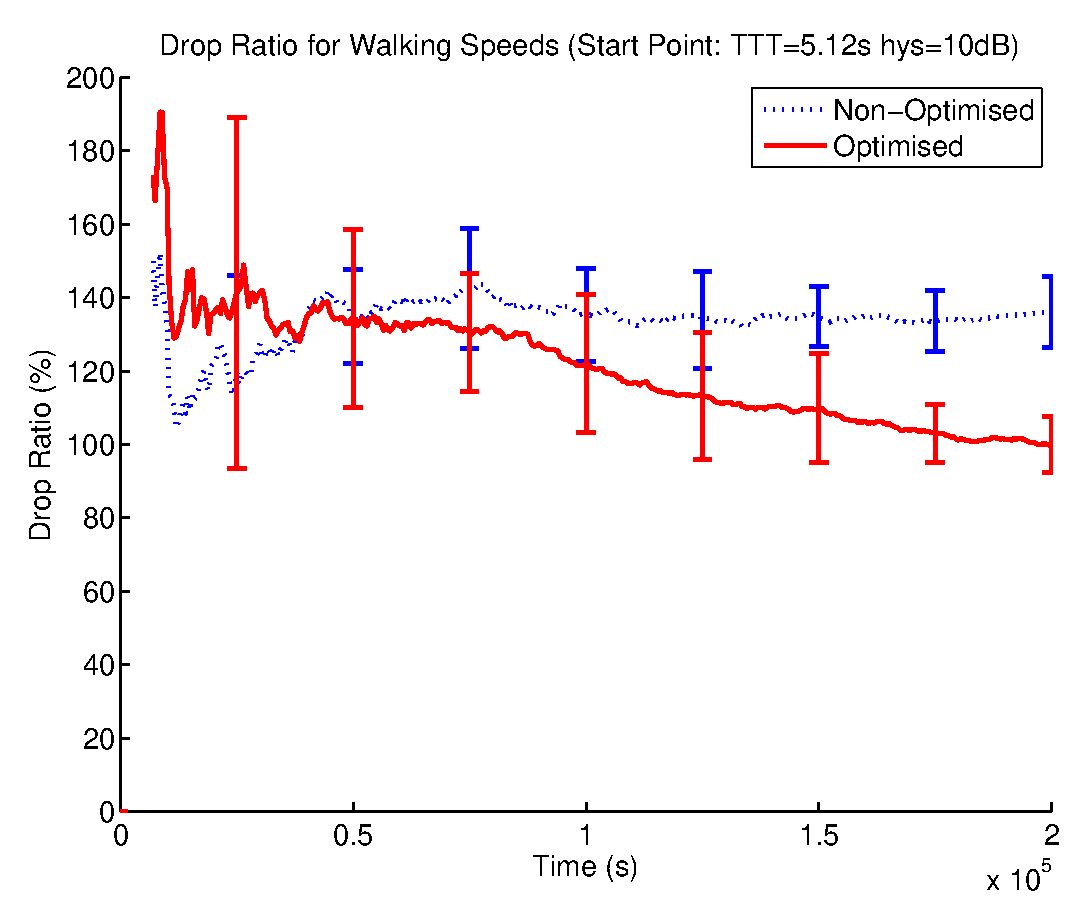
\includegraphics[width=0.66\textwidth]{figures/walking_figures/walkhigh.eps}
    \end{center}
    \caption{Graph of Optimised vs. Non-Optimised Results for Starting Point TTT=5.12s hys=10dB when UE traveling at walking speeds.}
    \label{fig:walk_high_drop}
\end{figure}
Figure~\ref{fig:walk_high_ttt} shows how the TTT values were optimised over the course of the simulation run. It can be seen that all the base stations were in consensus that 5.12 seconds is too large of a values of the TTT and very quickly lowered the value. After this however there were effectively two different groups. The first group made up of base stations 1, 3, 4 and 5 ended up keeping the TTT value over 1 second. While the other group made up of base stations 0, 2, 6, 7 and 8 kept reducing the value to a most 0.48 seconds. It could be said that first group of base stations may not have optimised the TTT value as well as the second group because it can be seen that base stations 1, 4 and 5 kept switching between only two values when dropped calls occurred. It can also be seen the these changes happened often meaning that these base stations were still have dropped calls occurring, so it cannot be said that these values performed as well as those the base stations is the second group were using.
While the changes made to the TTT value could be split up into two different groups the same cannot be said for the changes made to the hys value as seen in Figure~\ref{fig:walk_high_hys}. It can be seen that while most of the base stations kept the hys value above 9 dB, base stations 0, 6, 7 and 8 lower the value more, with base station 8 settling between 5 and 5.5 dB. It can also be seen that base stations 1 and 3 appear to have gotten stuck between two non-optimal values as they keep switching between them and due to it happening often it means that dropped calls are still occurring so the system should have switched to different values to see if they had performed better.
\begin{figure}[H]
        \centering
        \begin{subfigure}[b]{0.49\textwidth}
                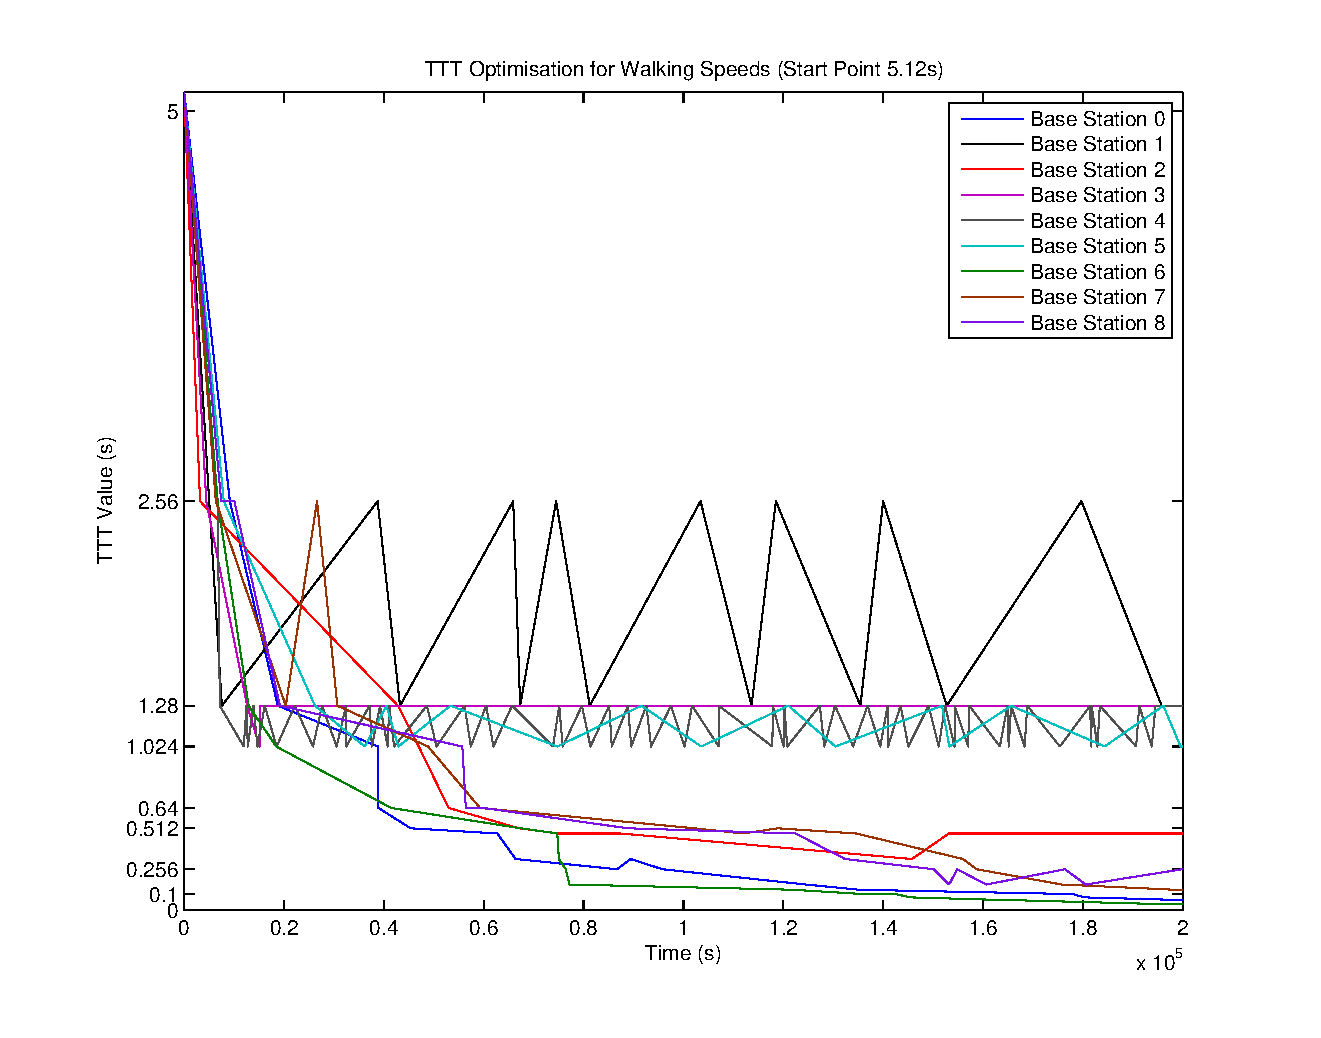
\includegraphics[width=\textwidth]{figures/walking_figures/high/long_ttt.eps}
                \caption{Changing TTT Values}
                \label{fig:walk_high_ttt}
        \end{subfigure}%
        ~ %add desired spacing between images, e. g. ~, \quad, \qquad etc.
          %(or a blank line to force the subfigure onto a new line)
        \begin{subfigure}[b]{0.49\textwidth}
                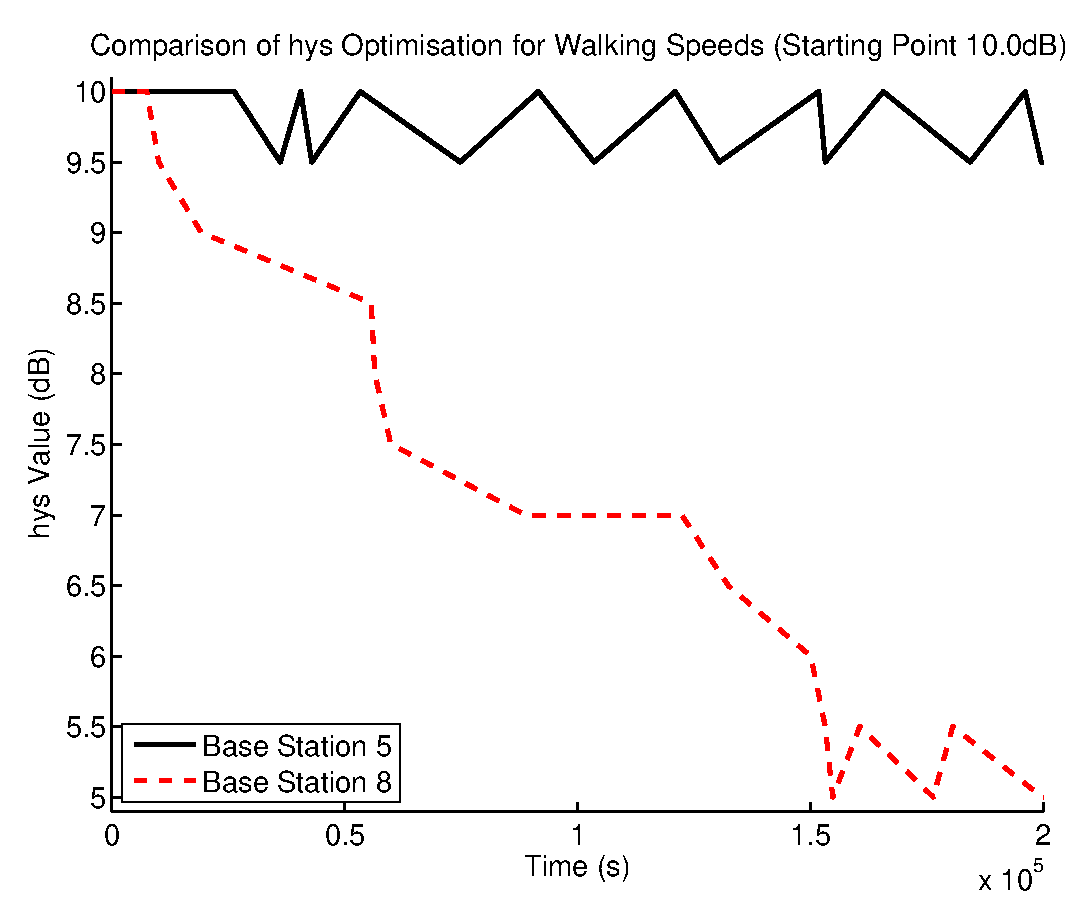
\includegraphics[width=\textwidth]{figures/walking_figures/high/long_hys.eps}
                \caption{Changing hys Values}
                \label{fig:walk_high_hys}
        \end{subfigure}
        \caption{Illustration of how the TTT and hys values changed over time for large values when UE traveling at walking speeds.}\label{fig:walk_high_ttthys}
\end{figure}
From these results it can be said that the system performed as expected by reducing both the TTT and hys in the case of all the base stations. There were also a very high number for dropped calls and no ping-pong's, which was also expected in the simulation.
\subsection{Middle Starting Values}
Again as seen in Figure~\ref{fig:walk_mid_drop} the optimised values performed a lot better than the static values when they were originally set to the their middle values of 0.256 seconds for TTT and 5 dB for hys. The results also show that unlike with the results seen in Figure~\ref{fig:walk_high_drop} the optimisation process did not greatly increase the number of dropped call at first. Instead it was the non-optimised values that began with the large number of dropped calls. This means that when these dropped calls began to appear the machine learning algorithm changed the value of TTT and hys in such a way that the dropped calls seen for the non-optimised values did not happen.
\begin{figure}[H]
  \begin{center}
    	  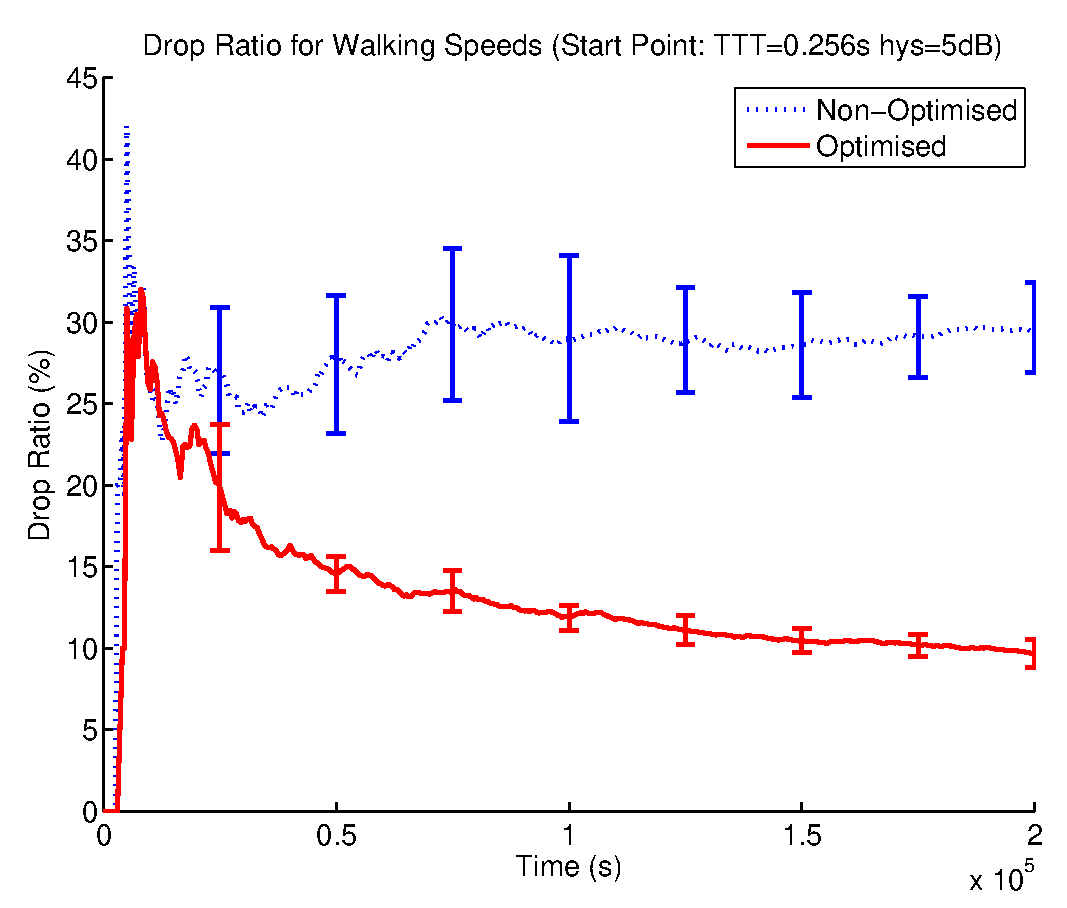
\includegraphics[width=0.75\textwidth]{figures/walking_figures/walkmid.eps}
    \end{center}
    \caption{Graph of Optimised vs. Non-Optimised Results for Starting Point TTT=0.256s hys=5dB when UE traveling at walking speeds.}
    \label{fig:walk_mid_drop}
\end{figure}
The way that the value of TTT trended during the simulation can be seen in Figure~\ref{fig:walk_mid_ttt}. It can be seen that the majority of the base stations ended up having the TTT being 0.1 seconds with those base stations having very few changes from that value when they got there meaning that it could be an optimal value. As expected base station 4 came up with a different solution to the other base stations by actually increasing the value of TTT when the majority were reducing it.

Figure~\ref{fig:walk_mid_hys} shows that all but one base station were in consensus that the value of hys should be lowered from its starting value. Other than this though there was not very much consensus with the base stations finishing with any value in the range of 2.5 to 4 dB.

It is interesting to note that base station 8 actually ended up switching between the same states of values TTT=0.256 seconds hys=5 dB and TTT=0.16 seconds and hys=5.5 dB by the end of both simulations for starting at large and middle values. This means that these could be the most optimal states found for the base station.
\begin{figure}[H]
        \centering
        \begin{subfigure}[b]{0.49\textwidth}
                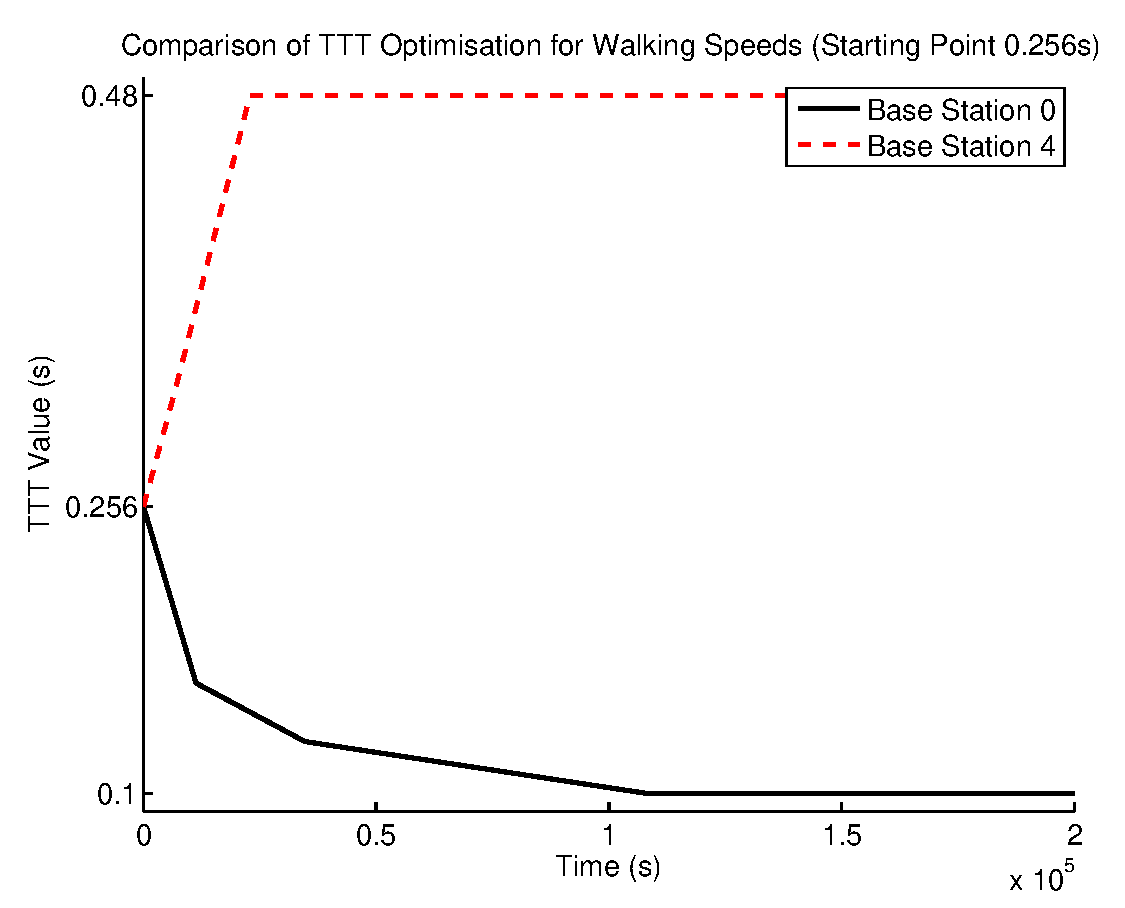
\includegraphics[width=\textwidth]{figures/walking_figures/mid/long_ttt.eps}
                \caption{Changing TTT Values}
                \label{fig:walk_mid_ttt}
        \end{subfigure}%
        ~ %add desired spacing between images, e. g. ~, \quad, \qquad etc.
          %(or a blank line to force the subfigure onto a new line)
        \begin{subfigure}[b]{0.49\textwidth}
                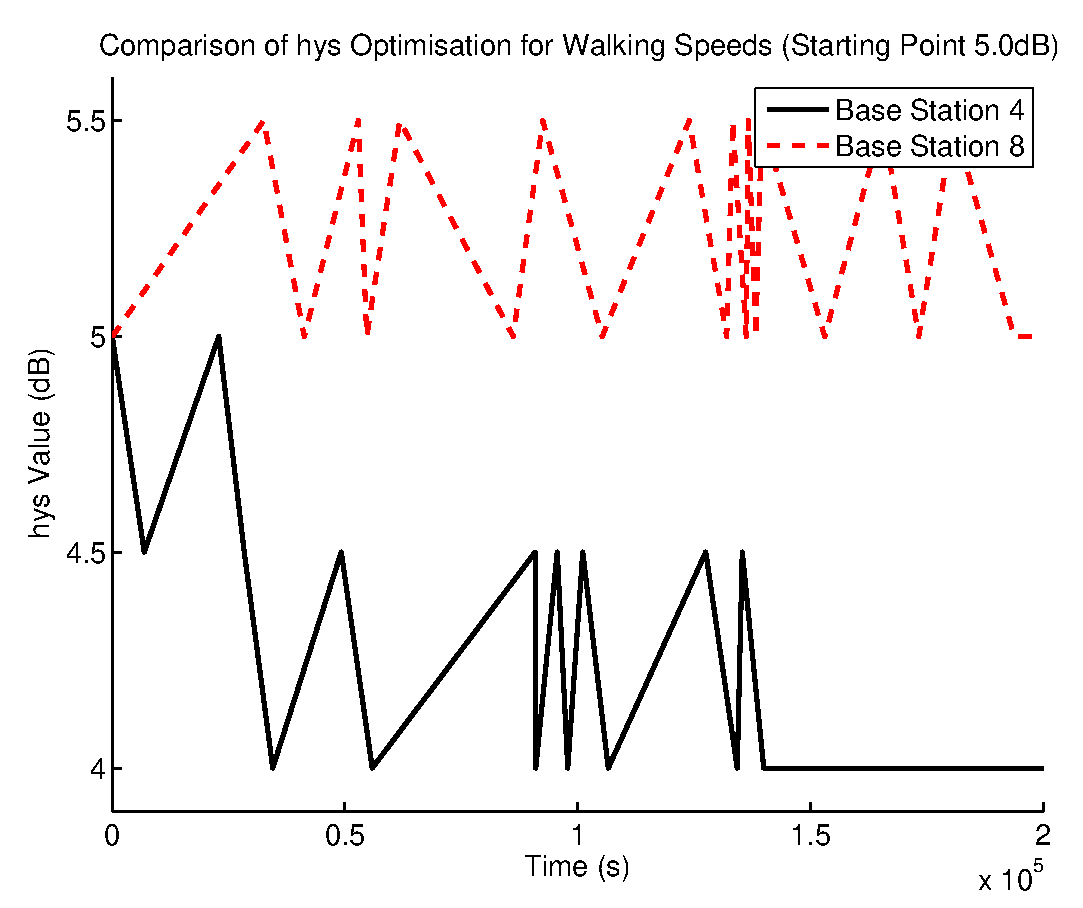
\includegraphics[width=\textwidth]{figures/walking_figures/mid/long_hys.eps}
                \caption{Changing hys Values}
                \label{fig:walk_mid_hys}
        \end{subfigure}
        \caption{Illustration of how the TTT and hys values changed over time for medium values when UE traveling at walking speeds.}\label{fig:walk_mid_ttthys}
\end{figure}
The system performed as expected in this scenario with the majority of the base stations reducing both the TTT and hys to attempt to improve the performance. Some base stations, however, took an unexpected approach by actually increasing the values.
\subsection{Small Starting Values}
It turned out that ping-pong's were a very rare occurrence in the simulation. This was most likely due to there being no fading in the simulation and that Random Direction mobility model would having the UE moving in one direction for a long time meaning that the only likely occurrence of a ping-pong would be if a handover took place and the UE then turned around and moved the other direction.

Figure~\ref{fig:walk_low_ping} shows how the optimisation system performed against the static values when the simulation started with the TTT being 0 seconds and the hys being 0 dB. It can be seen that the optimised values only actually began to perform better than the static values at the very end of the simulation run. However, it can also be seen the ping-pong ratio for the static values was actually trending up while the ratio for the optimised values was trending down. This means that long term the optimised values should perform much better. 
\begin{figure}[H]
  \begin{center}
    	  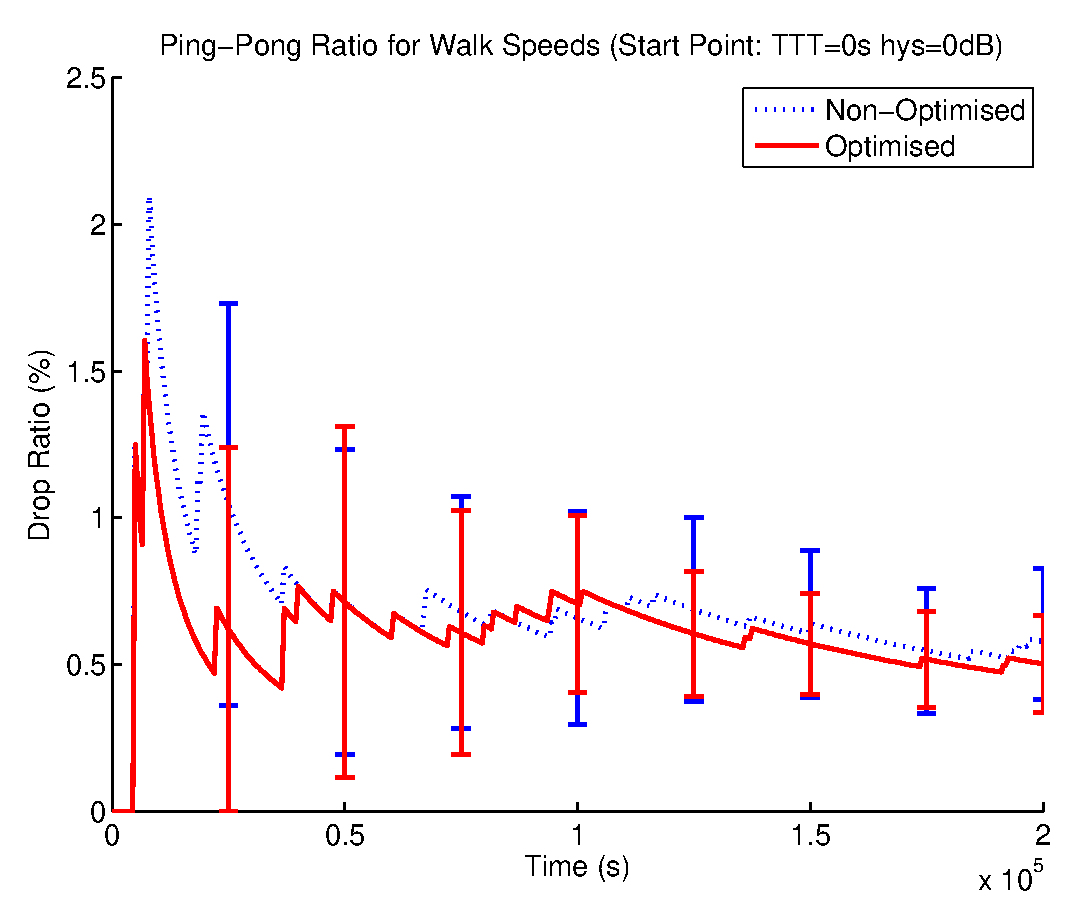
\includegraphics[width=0.75\textwidth]{figures/walking_figures/walklow.eps}
    \end{center}
    \caption{Graph of Optimised vs. Non-Optimised Results for Starting Point TTT=0s hys=0dB when UE traveling at walking speeds.}
    \label{fig:walk_low_ping}
\end{figure}
As for how the TTT and hys values changed over the simulation run in can be seen in Figure~\ref{fig:walk_low_ttt} that all the base stations were in consensus to keep to the TTT value at 0 seconds. This only changed at the very end of the run when base station 5 decided to increase the value to 0.04 seconds.

It can also be seen in Figure~\ref{fig:walk_low_hys} that the majority of the base stations were in consensus that the hys should have been increase to 0.5 dB. However, this change was made at differing times because due to pong-ping’s happening so rarely and the optimisation system only making changes when something goes wrong.
\begin{figure}[H]
        \centering
        \begin{subfigure}[b]{0.49\textwidth}
                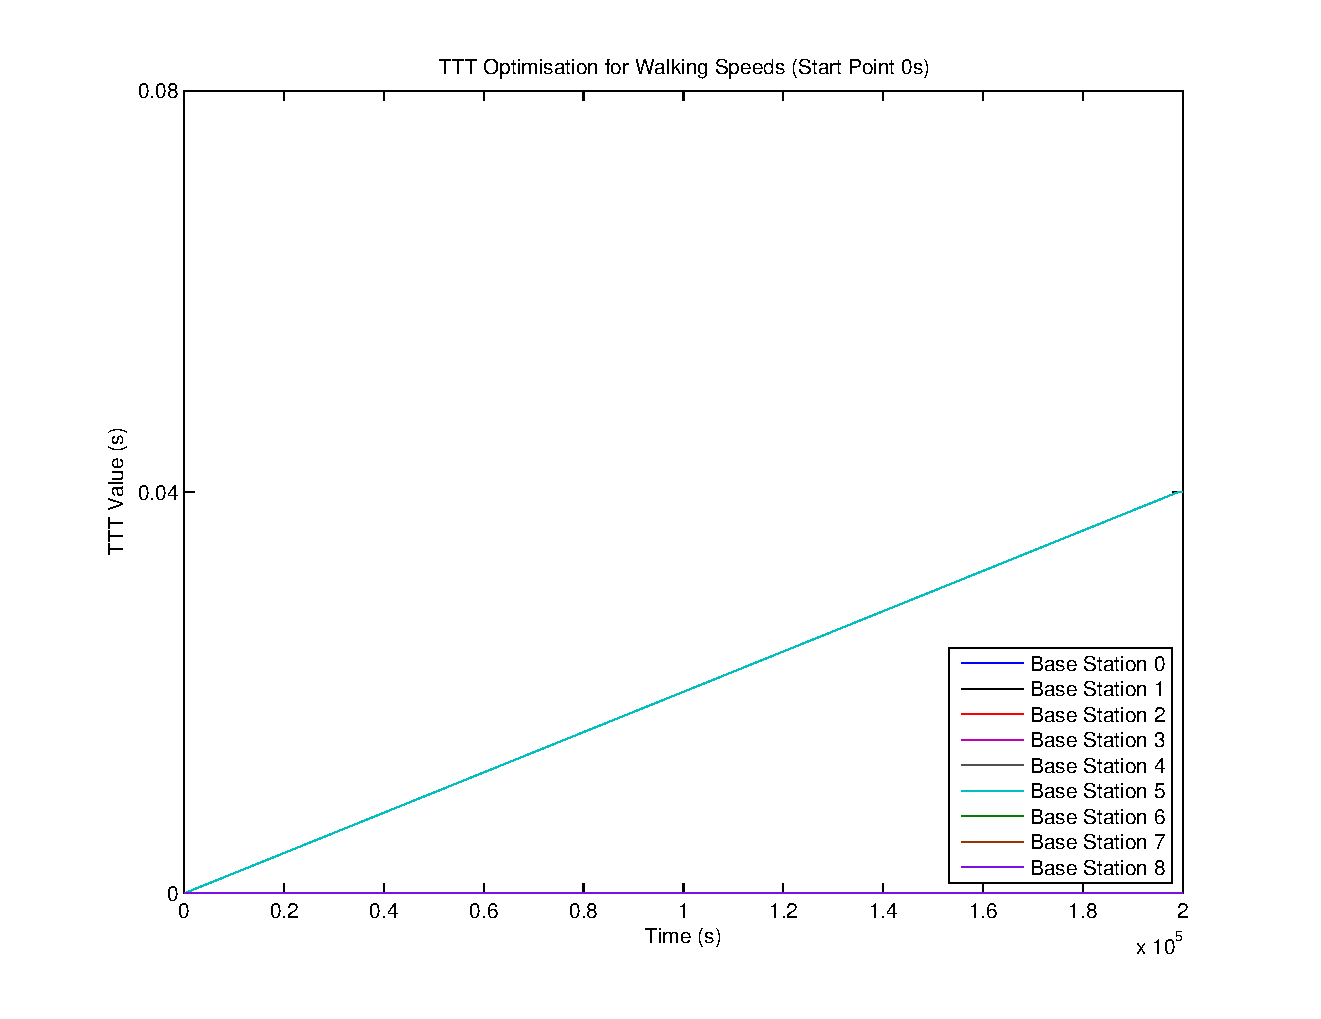
\includegraphics[width=\textwidth]{figures/walking_figures/low/long_ttt.eps}
                \caption{Changing TTT Values}
                \label{fig:walk_low_ttt}
        \end{subfigure}%
        ~ %add desired spacing between images, e. g. ~, \quad, \qquad etc.
          %(or a blank line to force the subfigure onto a new line)
        \begin{subfigure}[b]{0.49\textwidth}
                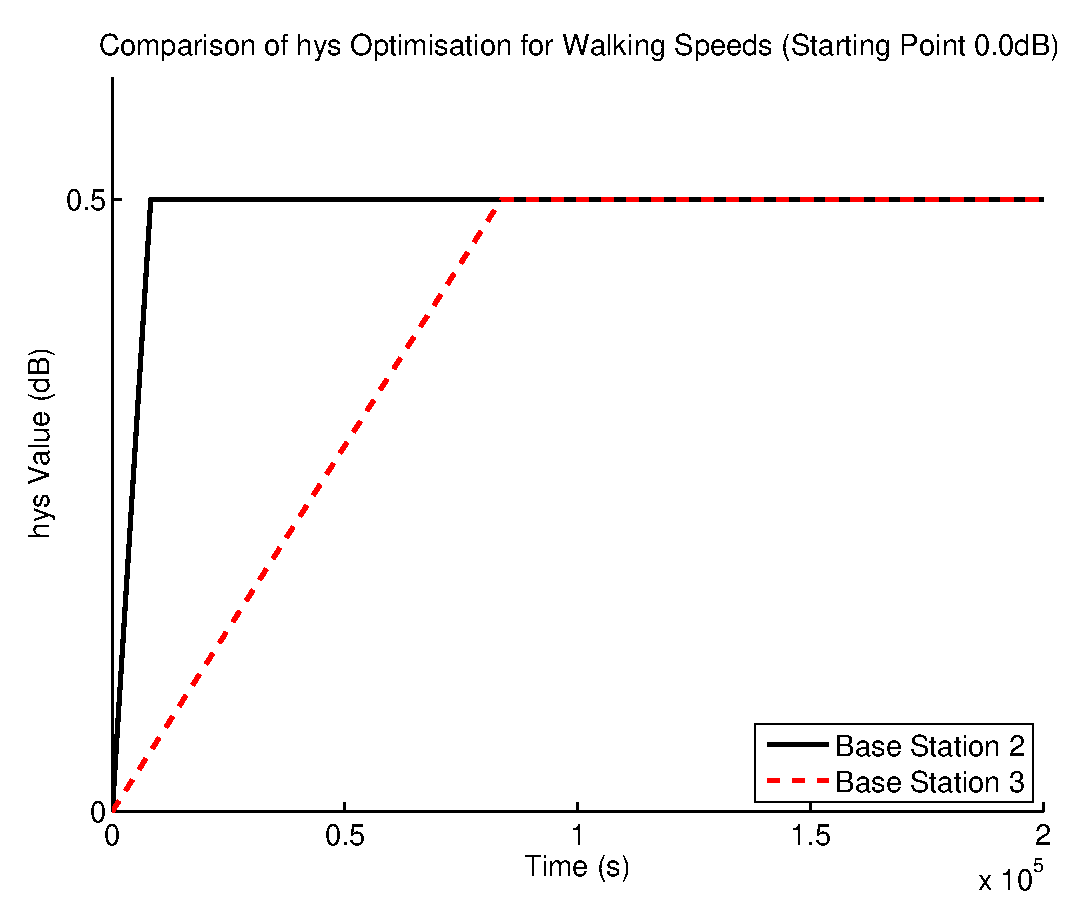
\includegraphics[width=\textwidth]{figures/walking_figures/low/long_hys.eps}
                \caption{Changing hys Values}
                \label{fig:walk_low_hys}
        \end{subfigure}
        \caption{Illustration of how the TTT and hys values changed over time for medium values when UE traveling at walking speeds.}\label{fig:walk_low_ttthys}
\end{figure}
This scenario played out as expected with no dropped calls occurring; instead having ping-pong’s determine the performance of the system. The system also compensated for this as expected by increase the value of the hys in most cases and by the end of the simulation run the performance of the optimised values had become better than that of the non-optimised values.
\subsection{Large hys and Small TTT Starting Values}
Much like the first three scenarios, it can be seen in Figure~\ref{fig:walk_highhys_drop} that, the optimised values performed better than the static values when the TTT and hys started at 0.08 seconds and 7.5 dB respectively. Also much like in the second scenario the optimisation process did not begin by greatly increasing the number of dropped when trying to optimise the values.
\begin{figure}[H]
  \begin{center}
    	  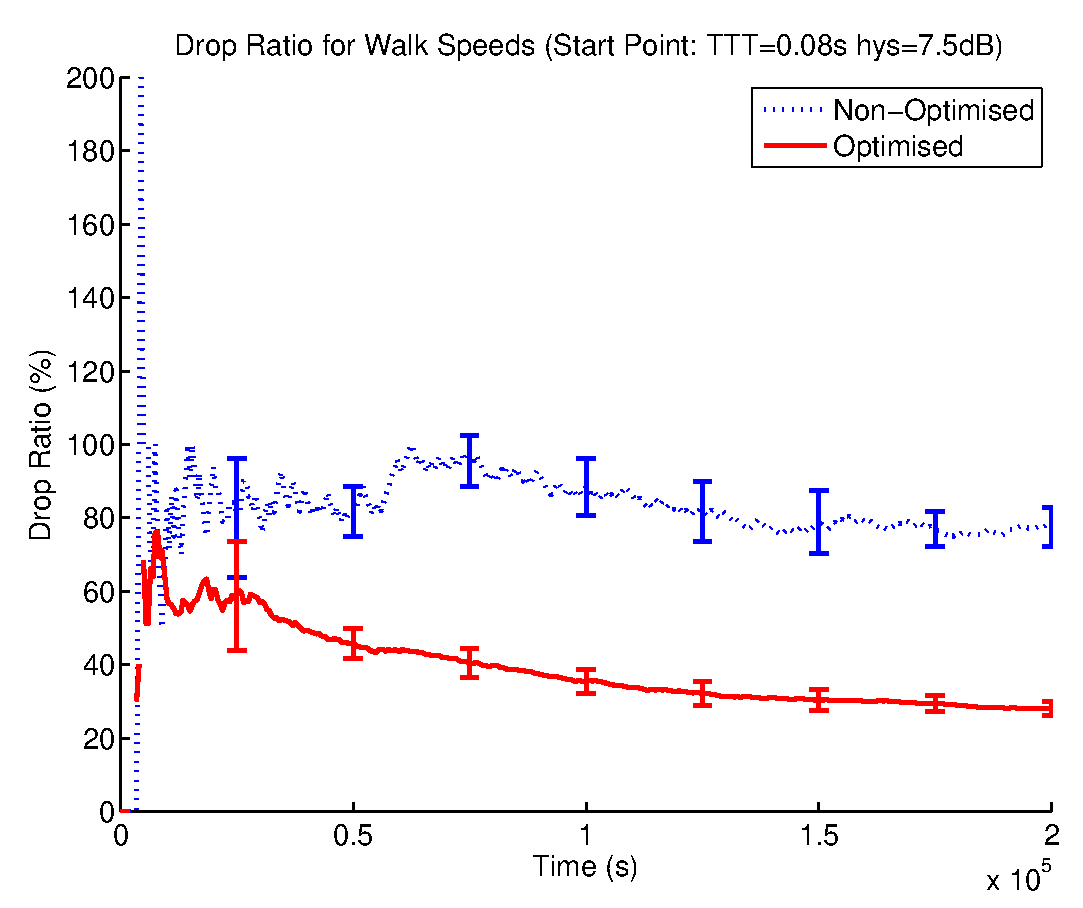
\includegraphics[width=0.75\textwidth]{figures/walking_figures/walkhighhys.eps}
    \end{center}
    \caption{Graph of Optimised vs. Non-Optimised Results for Starting Point TTT=0.08s hys=7.5dB when UE traveling at walking speeds.}
    \label{fig:walk_highhys_drop}
\end{figure}
The way in which the TTT values were changed during the optimisation process can be seen in Figure~\ref{fig:walk_highhys_ttt}. The figure shows that there was not very much consensus at all when it came to what value that TTT should be. It can also be seen that the value for the TTT for each base station was switching between the same two values a lot meaning that the optimisation system must having been making more changes to the value of the hys to try and get better performance.

Figure~\ref{fig:walk_highhys_hys} shows that while the base stations changed their value of hys quickly after the simulation began there is no real consensus a lot for what value would be most optimal. The majority of the base stations ended up after their own unique value for hys by the end of the simulation run with the values being in the range of 3.5 to 7.5 dB. While there was no consensus on what the value for hys should be it can also be seen that when the base stations settled on their own value of hys they stayed with it meaning that there probably should have been more changes made to the TTT value to improve the performance.
\begin{figure}[H]
        \centering
        \begin{subfigure}[b]{0.49\textwidth}
                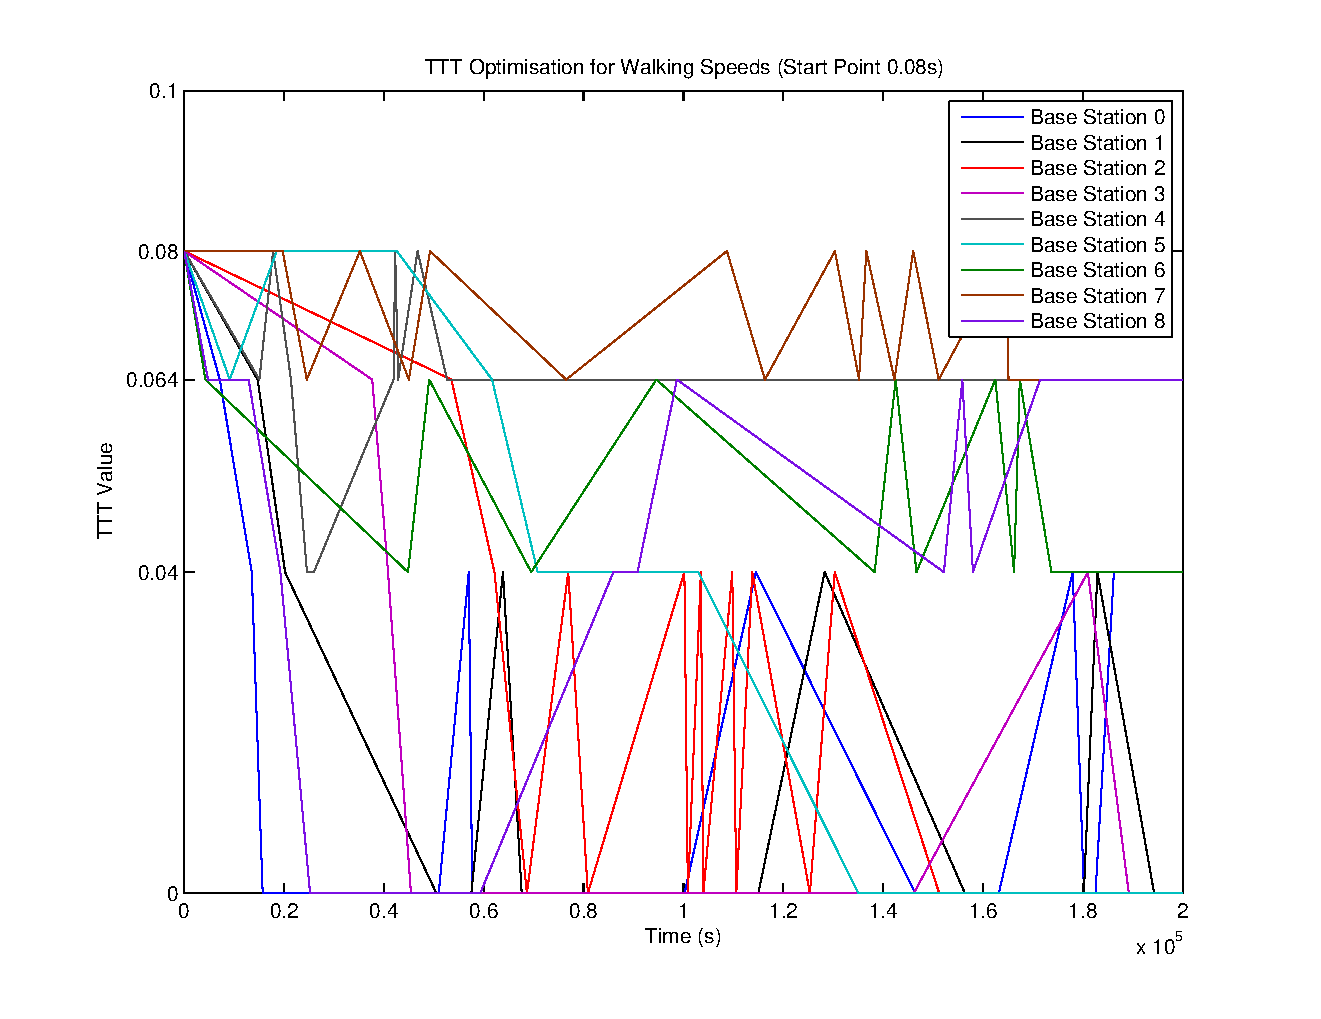
\includegraphics[width=\textwidth]{figures/walking_figures/highhys/long_ttt.eps}
                \caption{Changing TTT Values}
                \label{fig:walk_highhys_ttt}
        \end{subfigure}%
        ~ %add desired spacing between images, e. g. ~, \quad, \qquad etc.
          %(or a blank line to force the subfigure onto a new line)
        \begin{subfigure}[b]{0.49\textwidth}
                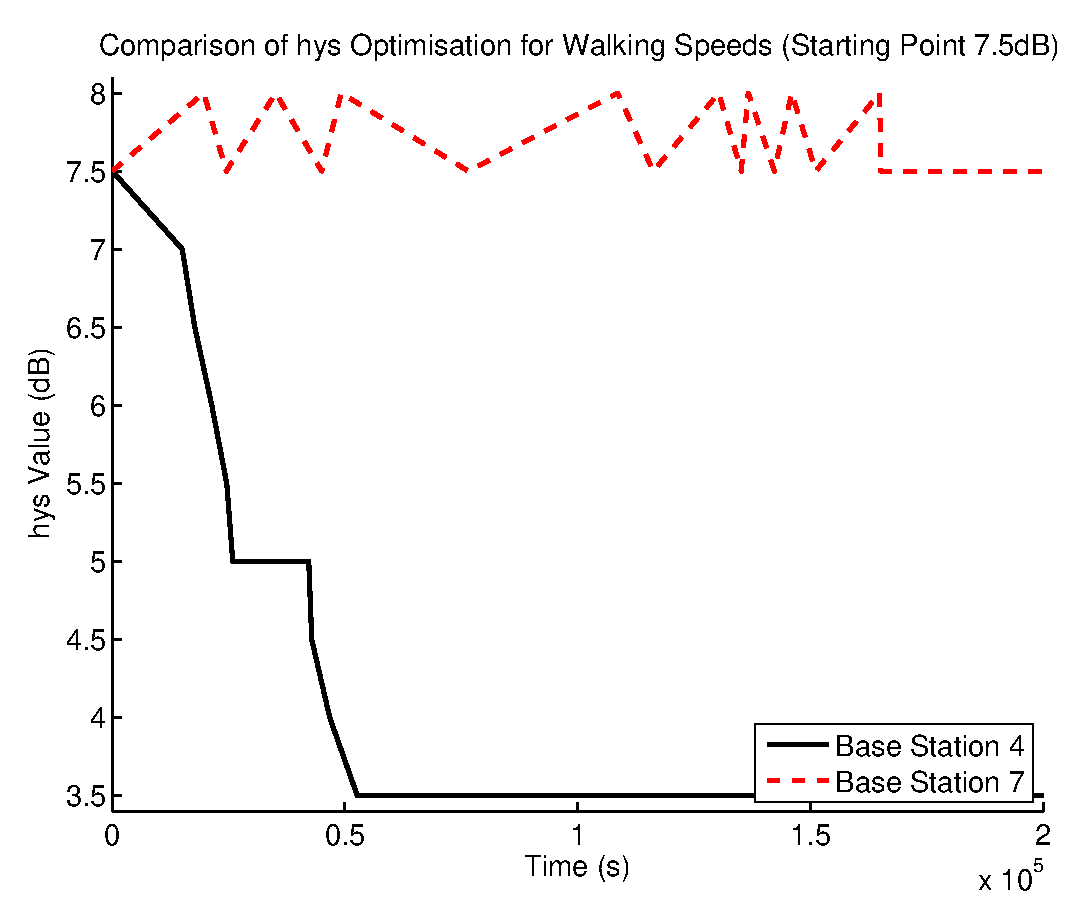
\includegraphics[width=\textwidth]{figures/walking_figures/highhys/long_hys.eps}
                \caption{Changing hys Values}
                \label{fig:walk_highhys_hys}
        \end{subfigure}
        \caption{Illustration of how the TTT and hys values changed over time for medium values when UE traveling at vehicle speeds.}\label{fig:walk_highhys_ttthys}
\end{figure}
In this scenario the system perform as expected in terms of decreasing the value of the hys. However, the system performed unexpectedly by also decreasing the value of the TTT when it was expected to actually increase it. Even with this the system still performed better than the simulation when run with static values.

\section{Vehicle Speed}
For the vehicle speed scenarios it is expected that number of dropped calls would increase over those seen in the walking speed scenarios due to the UE moving a lot faster and therefore giving a lot less time for the decision to handover or not. It is still expected that for the first scenario the system will reduce both values for TTT and hys. In the second scenario of the middle values it can also be expected the both values for TTT and hys will be reduced as dropped calls will still be expected fairly often at the speed the UE will be moving at. For the third scenario where both values for TTT and hys are at their lowest it is expected that the system will increase these values has ping-pong's should still be likely to happen, even at the high speeds. In the fourth scenario it is expected that the system is more likely to reduce both values, unlike when the UE was moving at walking speeds, because of the speed the UE is moving at decisions need to be made quickly.
\subsection{Large Starting Values}
It can be seen in Figure~\ref{fig:veh_high_drop} that the optimised system performed better than the system using the static values of 5.12 seconds for TTT and 10 dB for hys. 
\begin{figure}[H]
  \begin{center}
    	  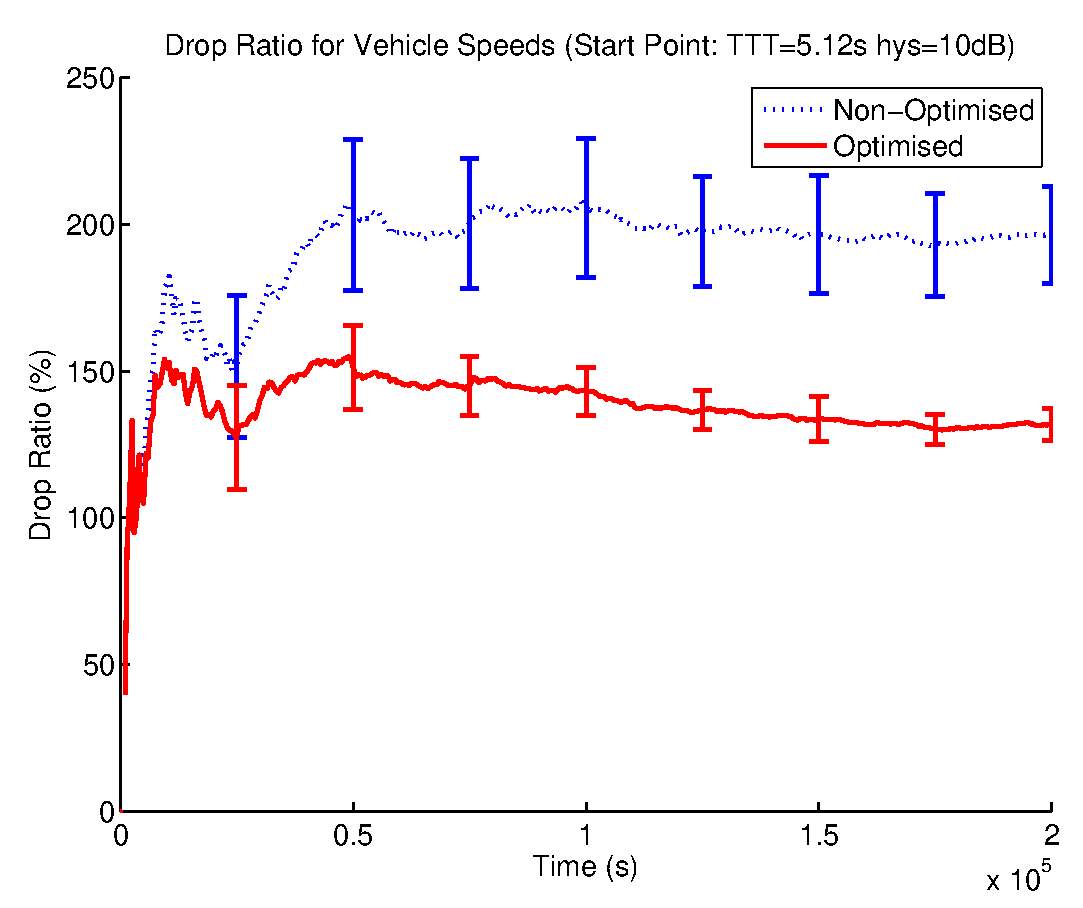
\includegraphics[width=0.75\textwidth]{figures/vehicle_figures/vehhigh.eps}
    \end{center}
    \caption{Graph of Optimised vs. Non-Optimised Results for Starting Point TTT=5.12s hys=10dB when UE traveling at walking speeds.}
    \label{fig:veh_high_drop}
\end{figure}
Figure~\ref{fig:veh_high_ttt} shows how the TTT value for the base stations changed over time. It can be seen that the system did not appear to optimise the value very well. A lot of the base stations kept switching between the values of 5.12 seconds and 2.56 seconds, which for a UE moving at roughly 30 mph is far too high and this is shown by the fact that the base stations are switching back and forth between the values almost constantly. This same kind of results can also be seen for the base stations that lowered the values slightly more, they are still switching between values very regularly meaning that the performance could have been improved a lot more. 

The same kind of results seen in the TTT values can also be seen in the hys in Figure~\ref{fig:veh_high_hys}. The results show that while some base stations managed to reduce the value of the hys as far down as 6 dB, the majority of the base stations kept the hys between 9 and 10 dB. This again looks to be far too high when the UE is moving at 30 mph as the base stations are constantly switching value but the performance never really improves.
\begin{figure}[H]
        \centering
        \begin{subfigure}[b]{0.49\textwidth}
                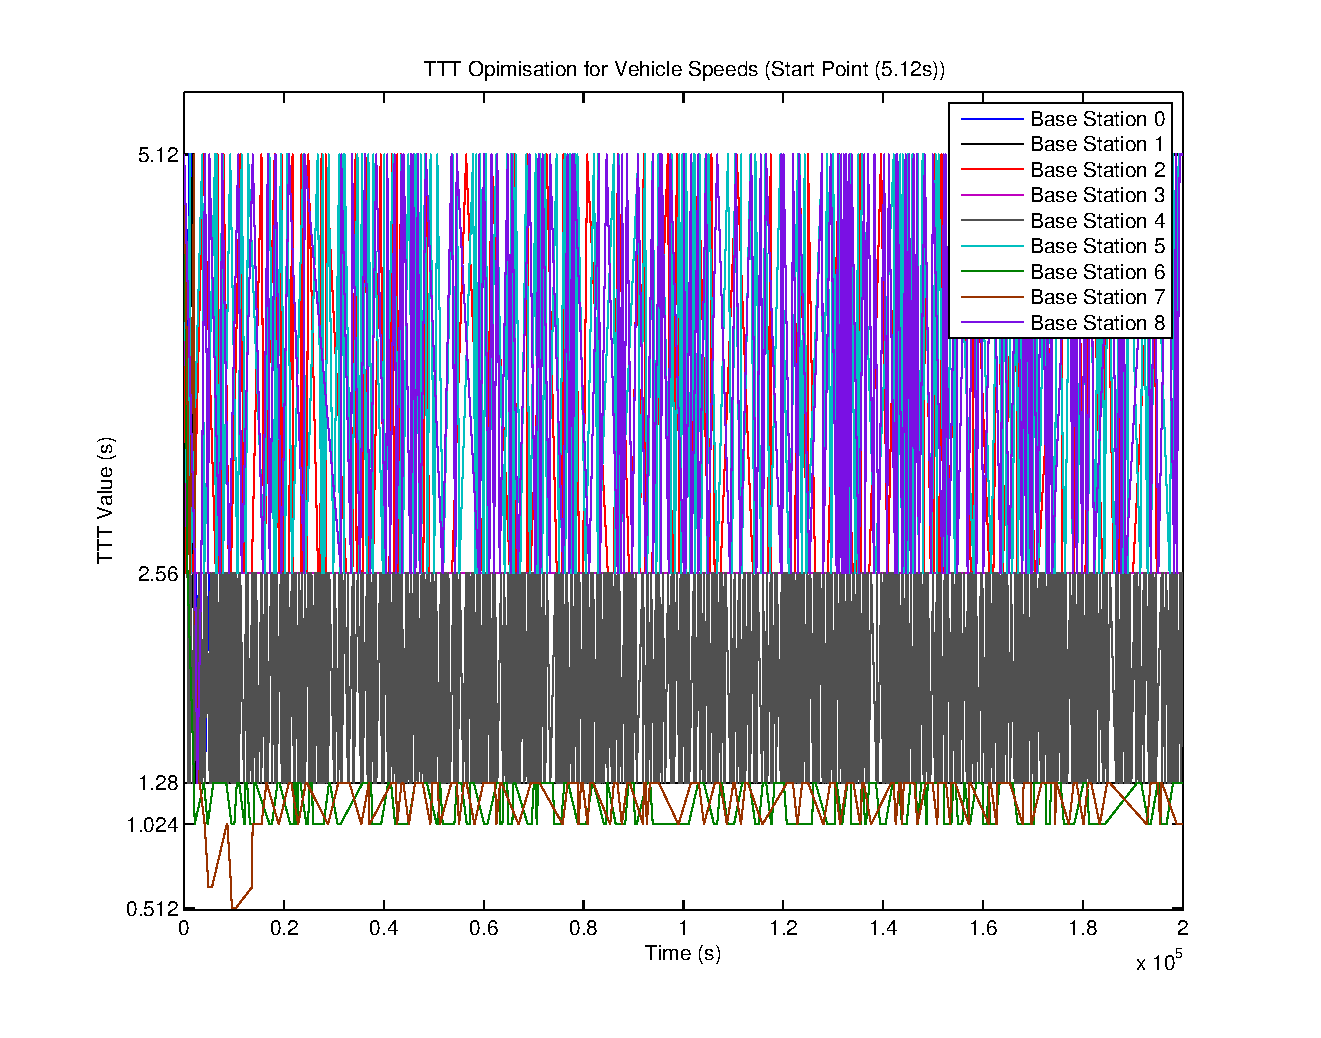
\includegraphics[width=\textwidth]{figures/vehicle_figures/high/long_ttt.eps}
                \caption{Changing TTT Values}
                \label{fig:veh_high_ttt}
        \end{subfigure}%
        ~ %add desired spacing between images, e. g. ~, \quad, \qquad etc.
          %(or a blank line to force the subfigure onto a new line)
        \begin{subfigure}[b]{0.49\textwidth}
                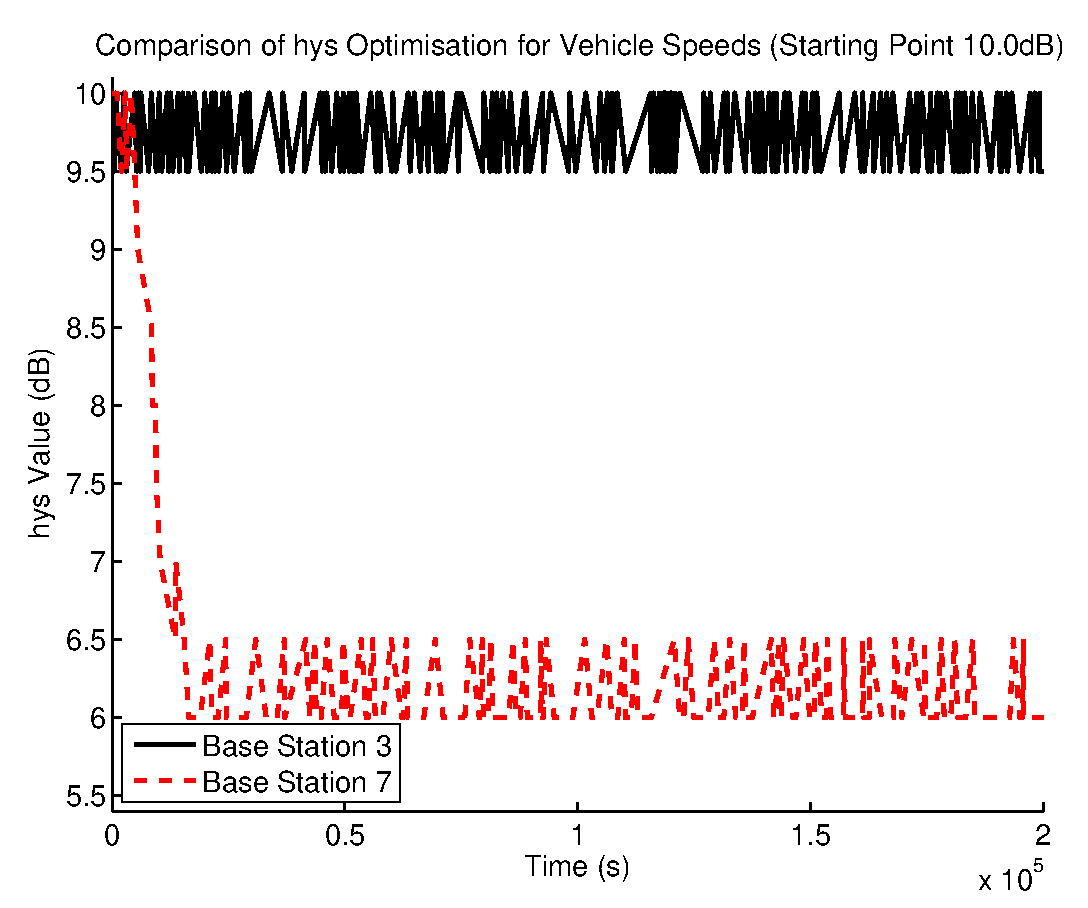
\includegraphics[width=\textwidth]{figures/vehicle_figures/high/long_hys.eps}
                \caption{Changing hys Values}
                \label{fig:veh_high_hys}
        \end{subfigure}
        \caption{Illustration of how the TTT and hys values changed over time for large values when UE traveling at vehicle speeds.}\label{fig:veh_high_ttthys}
\end{figure}
For this scenario while the system performed as expected and still performed better than that of the non-optimised system, it can be seen that it still did not perform all that well and appear be being getting stuck in non-optimal states.
\subsection{Middle Starting Values}
In this scenario the optimised system perform much better than of the static values, where it TTT and hys values were initialised to 0.256 seconds and 5 dB respectively. The graphs of the dropped calls ratios can be seen in Figure~\ref{fig:veh_mid_drop}.
\begin{figure}[H]
  \begin{center}
    	  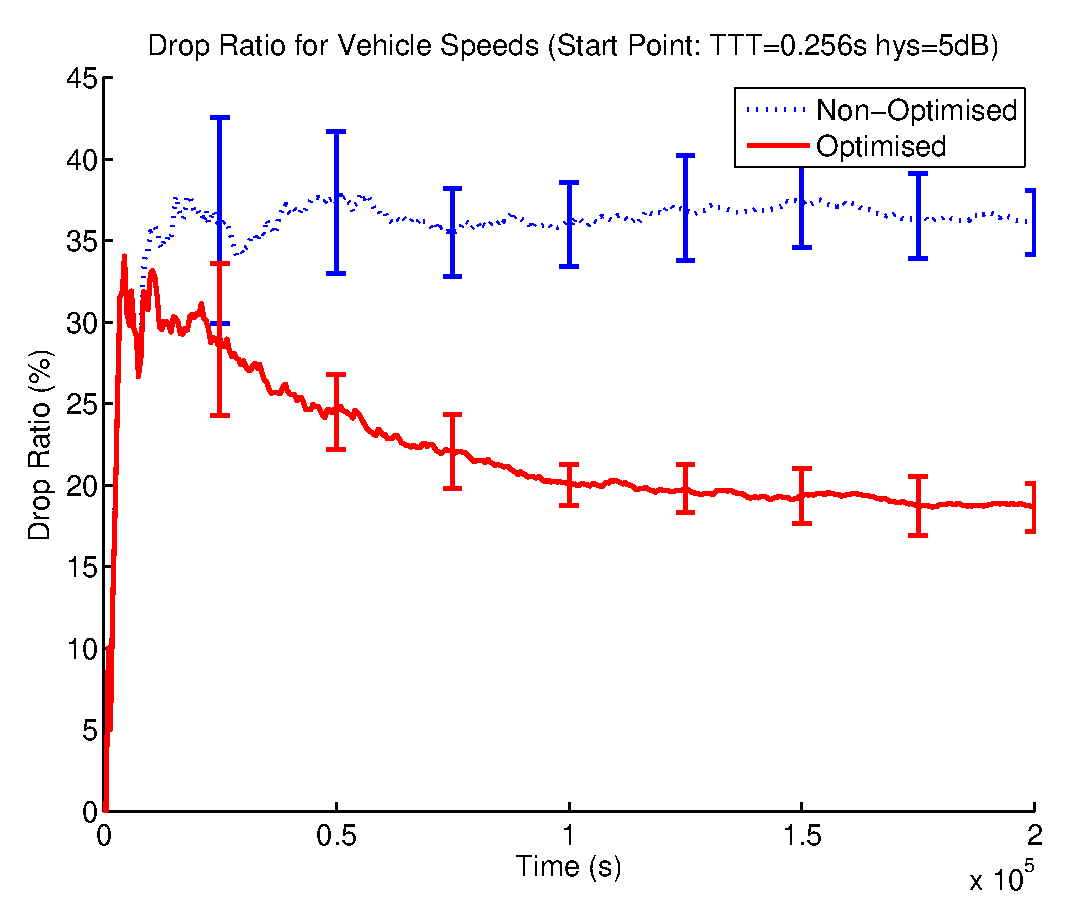
\includegraphics[width=0.75\textwidth]{figures/vehicle_figures/vehmid.eps}
    \end{center}
    \caption{Graph of Optimised vs. Non-Optimised Results for Starting Point TTT=0.256s hys=5dB when UE traveling at vehicle speeds.}
    \label{fig:veh_mid_drop}
\end{figure}
Figure~\ref{fig:veh_mid_ttt} shows how the TTT value for each base station changed over the time the simulation was run. It shows that most of the base stations lowered the value for TTT while base station 6 greatly increased the value. Although this large increase appears strange the base station did not have a far larger number of changes when compared to the other base stations, which means that the values performed just as well as the other values chosen by the other base stations. 

The way that the value for the hys was changed by the base stations can be seen in Figure~\ref{fig:veh_mid_hys}. It can be seen that the majority of the base stations kept the value of the hys around the starting point of 5 dB. Base station 4, however, reduced the value down to a minimum of 3.5 dB and be seen in have far less switches than the other base stations which means that it could have found a more optimal value.
\begin{figure}[H]
        \centering
        \begin{subfigure}[b]{0.49\textwidth}
                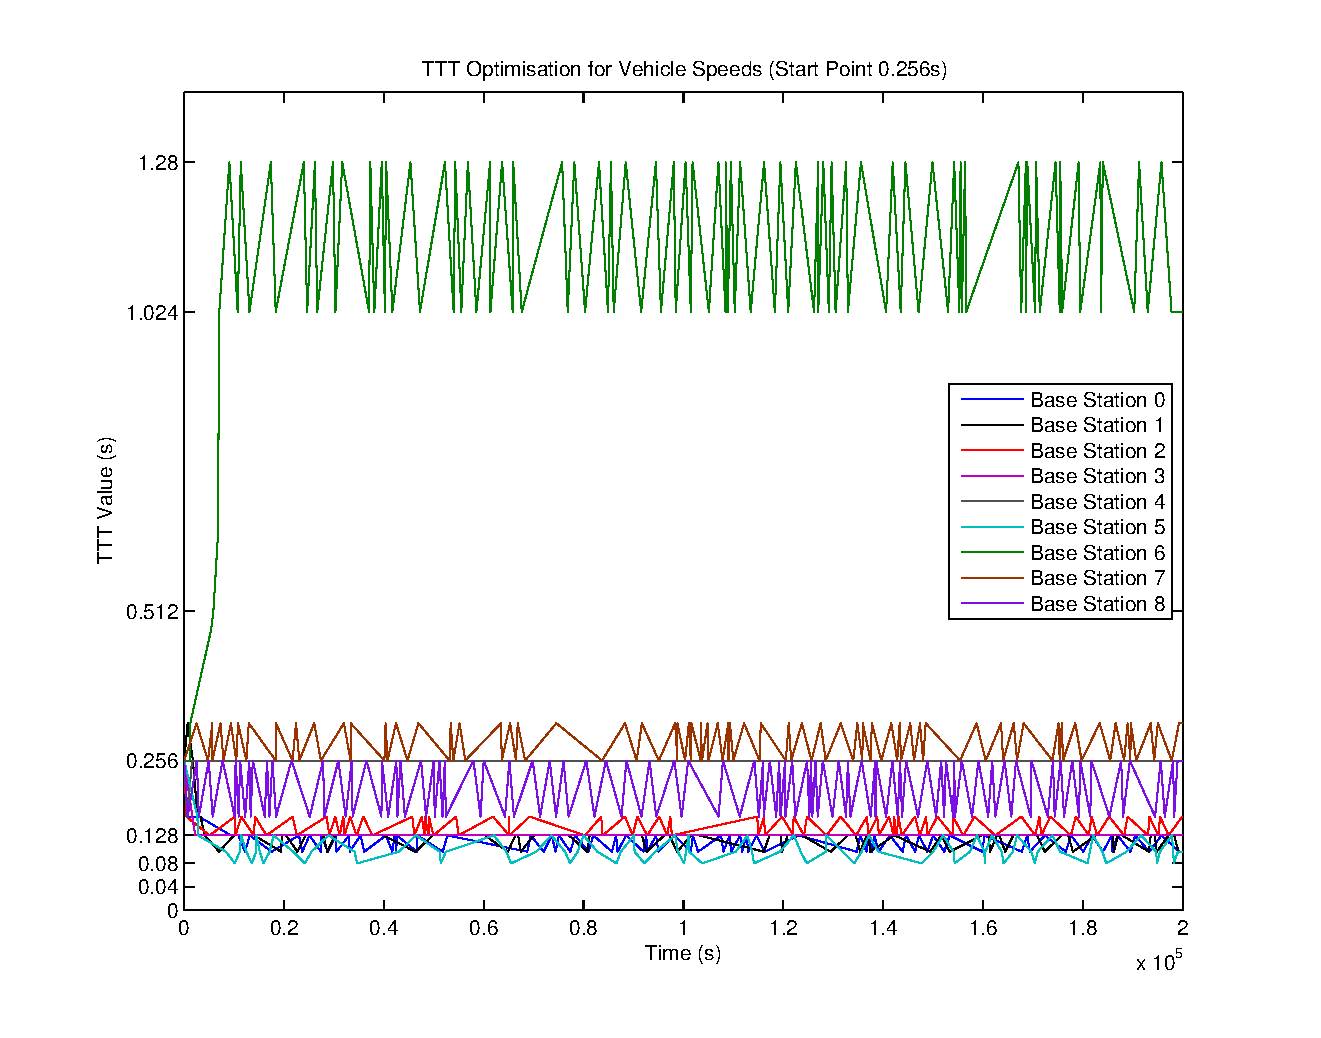
\includegraphics[width=\textwidth]{figures/vehicle_figures/mid/long_ttt.eps}
                \caption{Changing TTT Values}
                \label{fig:veh_mid_ttt}
        \end{subfigure}%
        ~ %add desired spacing between images, e. g. ~, \quad, \qquad etc.
          %(or a blank line to force the subfigure onto a new line)
        \begin{subfigure}[b]{0.49\textwidth}
                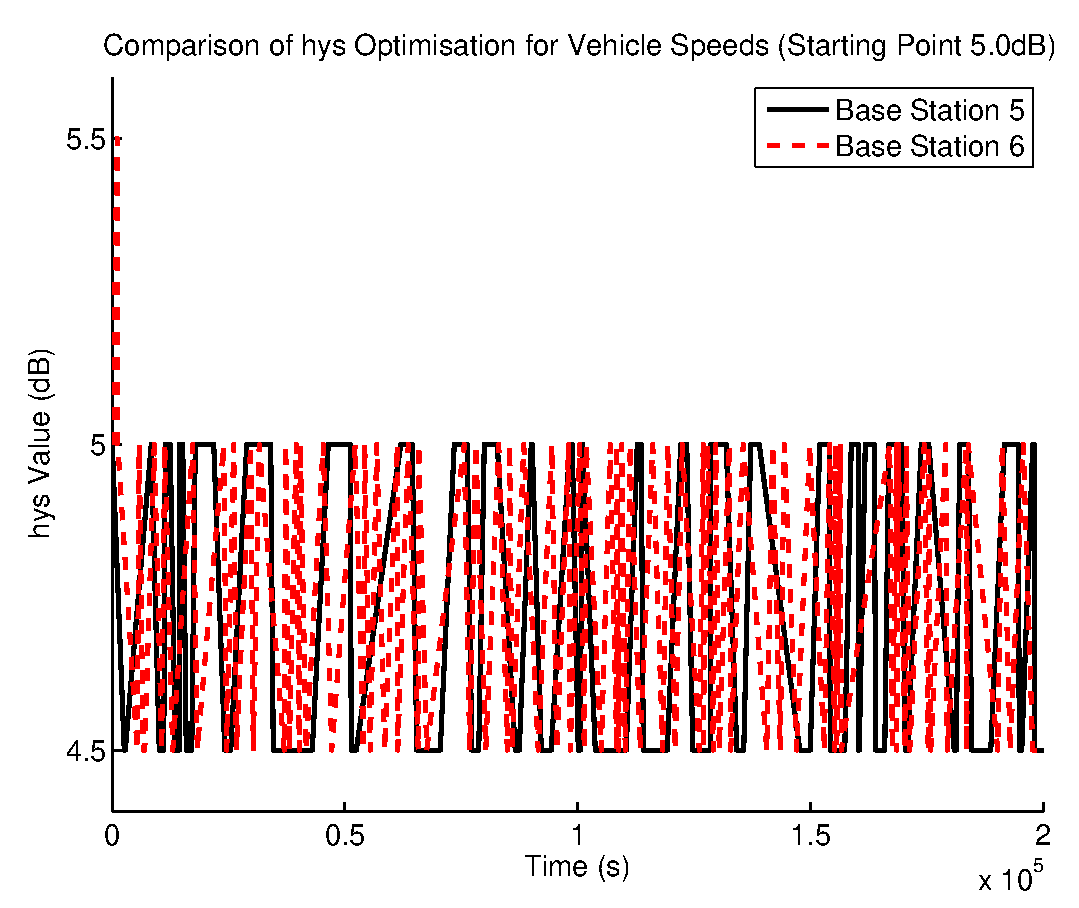
\includegraphics[width=\textwidth]{figures/vehicle_figures/mid/long_hys.eps}
                \caption{Changing hys Values}
                \label{fig:veh_mid_hys}
        \end{subfigure}
        \caption{Illustration of how the TTT and hys values changed over time for medium values when UE traveling at vehicle speeds.}\label{fig:veh_mid_ttthys}
\end{figure}
In this scenario it has been seen that the optimisation system functioned as expected with the majority of the base stations reducing both the TTT and hys values. However, there was a strange anomaly where one of the base stations greatly increased the TTT value, which was highly unexpected. 
\subsection{Small Starting Values}
It can be seen that for this scenario the optimised system performed well and even though at the beginning of the simulation it performed worse, by the end the ratio of ping-pong's was for better than that of the non-optimised values.
\begin{figure}[H]
  \begin{center}
    	  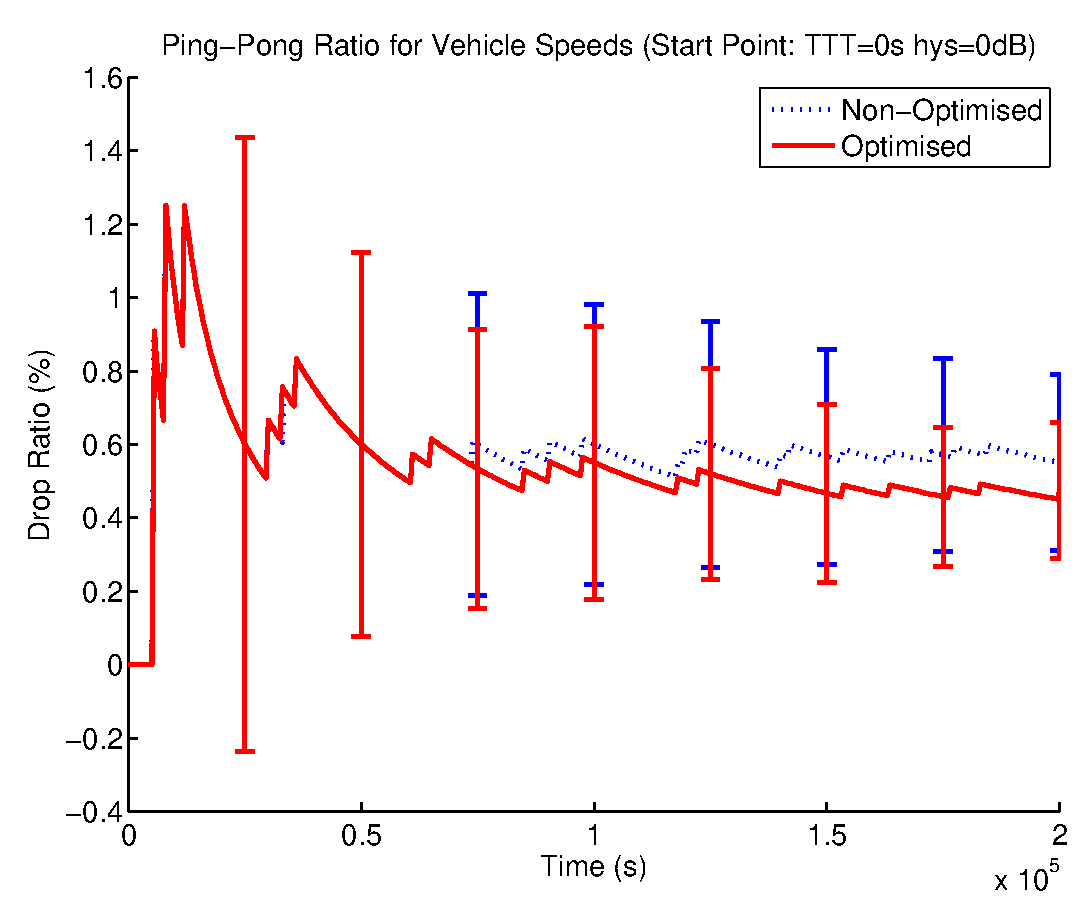
\includegraphics[width=0.75\textwidth]{figures/vehicle_figures/vehlow.eps}
    \end{center}
    \caption{Graph of Optimised vs. Non-Optimised Results for Starting Point TTT=0s hys=0dB when UE traveling at vehicle speeds.}
    \label{fig:veh_low_drop}
\end{figure}
Figure~\ref{fig:veh_low_ttt} shows of the TTT value for base stations were changed by the optimisation system. It can be seen that most of the base stations stayed with the value being 0 seconds while other tried increasing the value to 0.04 seconds, with two of the base stations actually going back down to 0 seconds afterwards.

Figure~\ref{fig:veh_low_hys} shows that the majority of the base stations increase the hys value 0.5 dB when a ping-pong occurred. Base station 3 actually increased the hys value to 1 dB when it had experienced two ping-pong’s. Even with this it still looks like 0.5 dB my have been the most optimal value for the situation.
\begin{figure}[H]
        \centering
        \begin{subfigure}[b]{0.49\textwidth}
                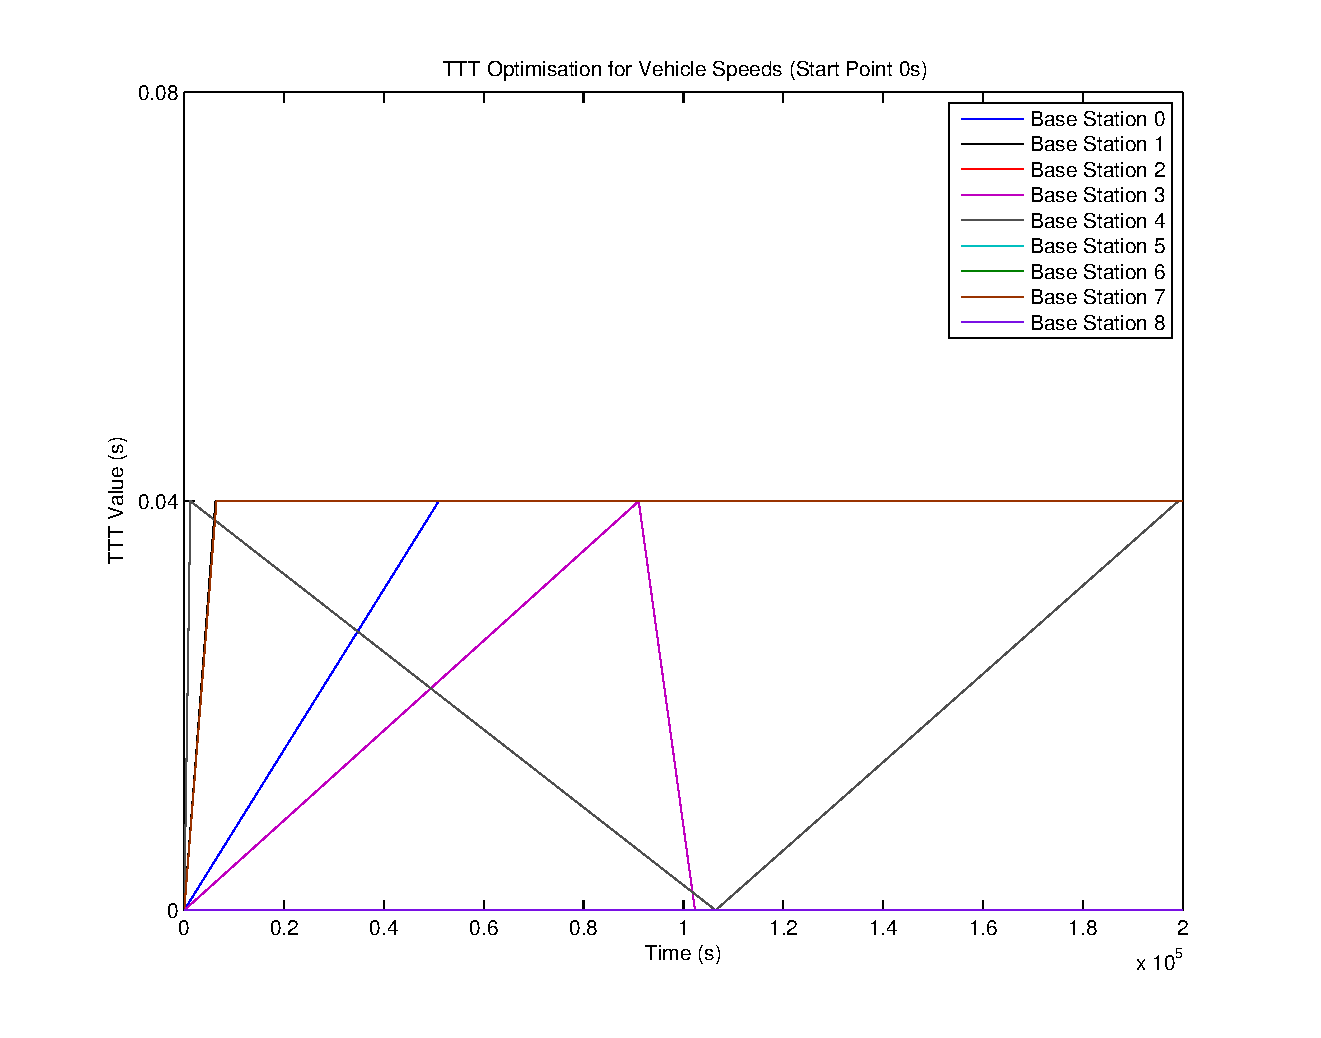
\includegraphics[width=\textwidth]{figures/vehicle_figures/low/long_ttt.eps}
                \caption{Changing TTT Values}
                \label{fig:veh_low_ttt}
        \end{subfigure}%
        ~ %add desired spacing between images, e. g. ~, \quad, \qquad etc.
          %(or a blank line to force the subfigure onto a new line)
        \begin{subfigure}[b]{0.49\textwidth}
                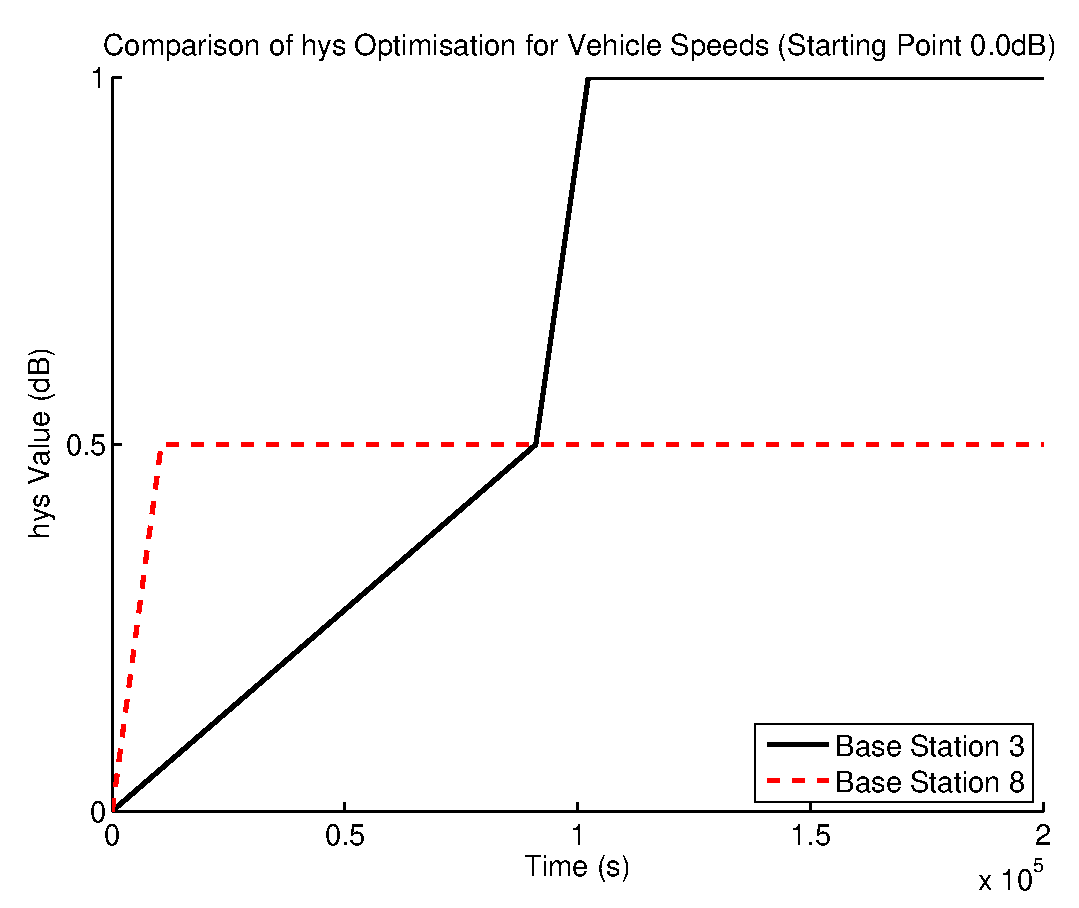
\includegraphics[width=\textwidth]{figures/vehicle_figures/low/long_hys.eps}
                \caption{Changing hys Values}
                \label{fig:veh_low_hys}
        \end{subfigure}
        \caption{Illustration of how the TTT and hys values changed over time for medium values when UE traveling at vehicle speeds.}\label{fig:vel_low_ttthys}
\end{figure}
Again the optimisation system functioned as expected with increasing both the TTT and hys values due to ping-pong’s occurring. This was expected because even though the UE is travel quickly the system still has to make sure that it does not trigger a handover too quickly.
\subsection{Large hys and Small TTT Starting Values}
As seen in the first three scenarios for the vehicle speed testing the optimised system managed to perform better than that of the non-optimised system when starting with the TTT being 0.08 seconds and the hys 7.5 dB. However, the improvement was not quite as great as seen in the other scenarios. 
\begin{figure}[H]
  \begin{center}
    	  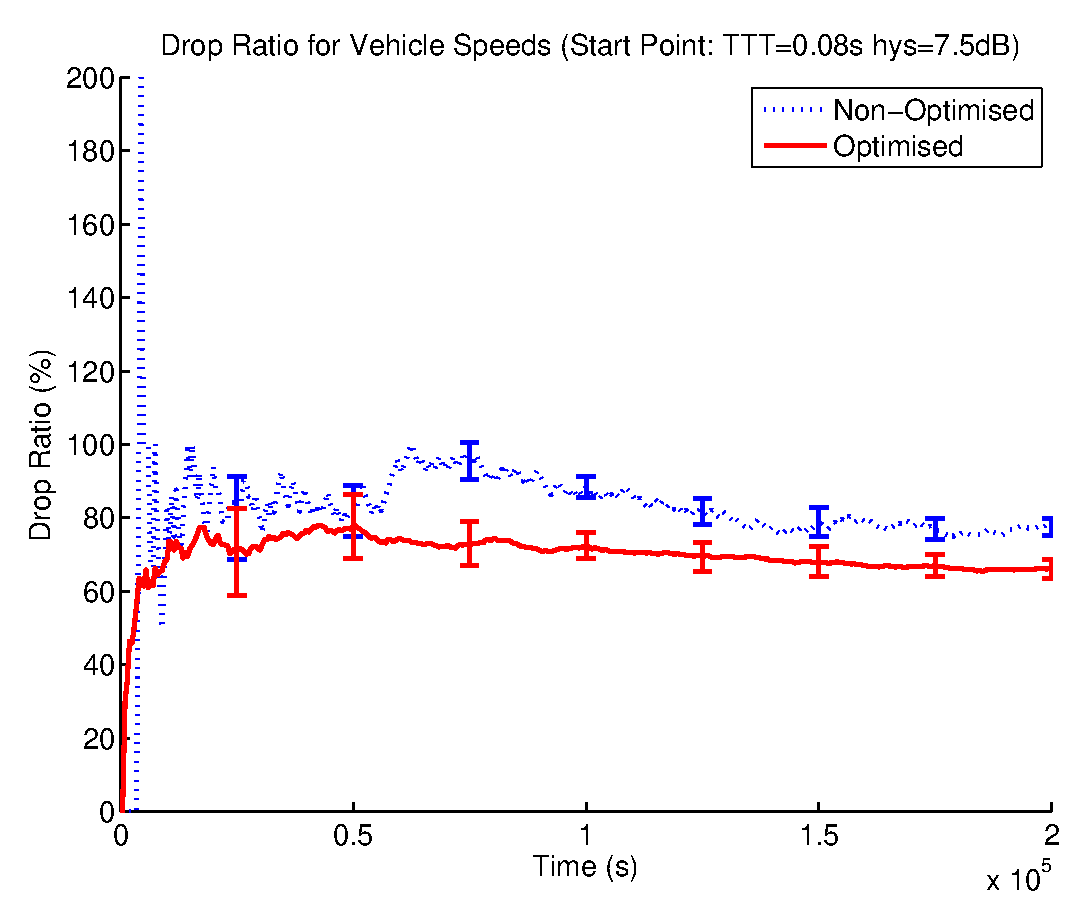
\includegraphics[width=0.75\textwidth]{figures/vehicle_figures/vehhighhys.eps}
    \end{center}
    \caption{Graph of Optimised vs. Non-Optimised Results for Starting Point TTT=0.08s hys=7.5dB when UE traveling at vehicle speeds.}
    \label{fig:veh_highhys_drop}
\end{figure}
It can be seen in Figure~\ref{fig:veh_highhys_ttt} that the base stations did not really come to a consensus on what should be done to the TTT when a dropped call occurs. Some of the base stations increased the value while others lowered it to as low as 0 seconds. It is also hard to tell if it was correct to either increase or decrease the value as all the base stations are constantly switching between values which means calls are still being dropped.

Much like with the results seen for how the TTT was changed, there is no real consensus that can be seen for changed the value for the hys as seen in Figure~\ref{fig:veh_highhys_hys}. It is seen that some base stations increased the value while other decreased it and only base station 0 decreased it by a large amount.
\begin{figure}[H]
        \centering
        \begin{subfigure}[b]{0.49\textwidth}
                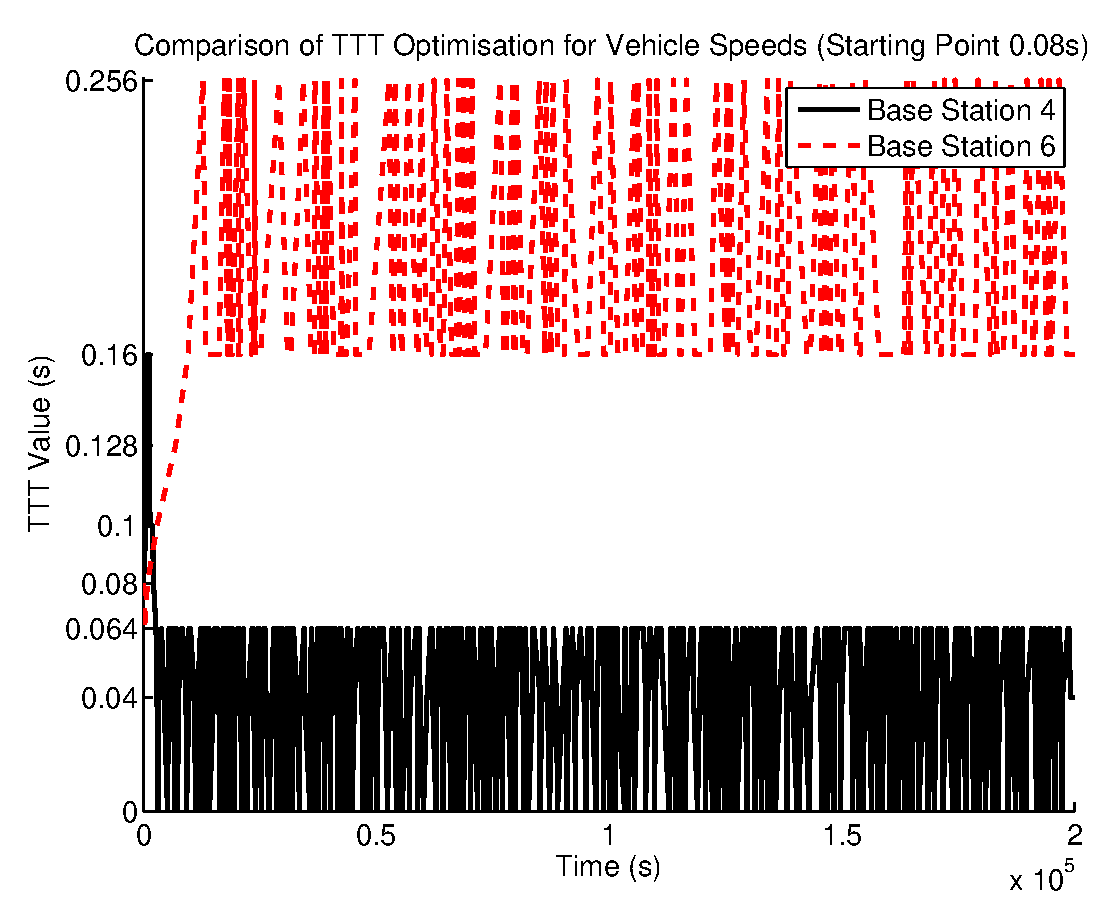
\includegraphics[width=\textwidth]{figures/vehicle_figures/highhys/long_ttt.eps}
                \caption{Changing TTT Values}
                \label{fig:veh_highhys_ttt}
        \end{subfigure}%
        ~ %add desired spacing between images, e. g. ~, \quad, \qquad etc.
          %(or a blank line to force the subfigure onto a new line)
        \begin{subfigure}[b]{0.49\textwidth}
                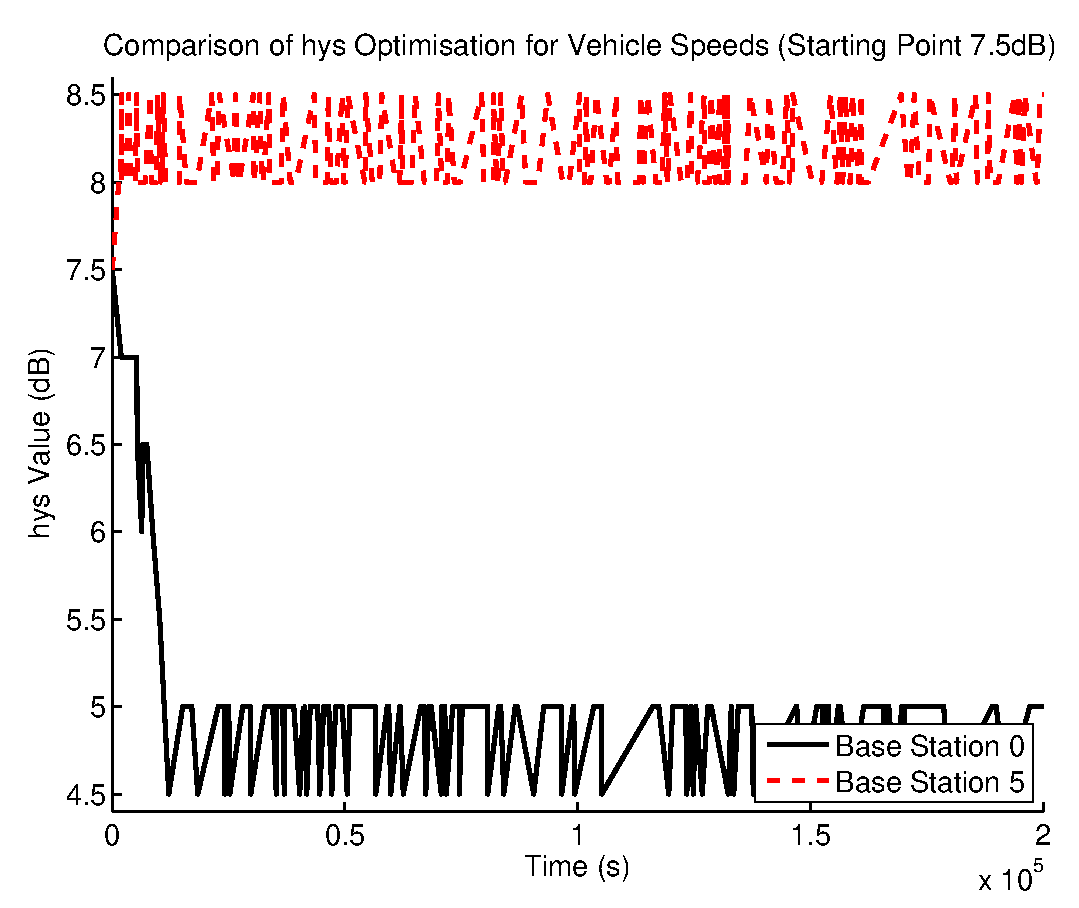
\includegraphics[width=\textwidth]{figures/vehicle_figures/highhys/long_hys.eps}
                \caption{Changing hys Values}
                \label{fig:veh_highhys_hys}
        \end{subfigure}
        \caption{Illustration of how the TTT and hys values changed over time for medium values when UE traveling at vehicle speeds.}\label{fig:veh_highhys_ttthys}
\end{figure}
Much like with the other scenarios it is seen that while the system may have been an improvement over the static values the system still could have performed far better, as base stations appeared to keep switching between values that could be considered non-optimal.
\section{Evaluation}
Over the four scenarios used to test the optimisation system for walking speeds it can be seen that overall the system performed better than if no optimisation was done at all. It can also be seen that the system makes improvements to the performance very quickly. As seen in scenarios for the middle values and the large hys with small TTT the system managed to not have the large spike in dropped calls at the beginning of their simulation runs which were seen in there respective non-optimised runs.

In the scenarios for vehicle speeds it was seen that the system did performed better than if no optimisation was used. However, it was seen in the ways that the TTT and hys values were changed that they did not stop dropped calls constantly happening, which means that these values were likely non-optimal. Therefore it is possible that the system could have performed a lot better if the system did not get stuck between non-optimal states.

It can, however, be seen that when the system does not get stuck between non-optimal states that it will optimise the TTT and hys values as quickly as it is needed, i.e., whenever a dropped call or ping-pong occurs.

The optimisation system, however, also appears to have some drawbacks. It was seen in the first scenario that the optimisation system caused a very large increase to the dropped call ratio before improving it. This is a usual downside in optimisation processes where 'things have to get worse before they can get better' and this process is a part of Q-Learning where the possible future rewards are taken into account when selecting a new state to move to. It was also seen in the scenarios using the vehicle speeds that the system appeared to keep getting stuck between two states that appear to be non-optimal which degrading the performance which had the potential to do a lot better.